\documentclass[]{book}
\usepackage{lmodern}
\usepackage{amssymb,amsmath}
\usepackage{ifxetex,ifluatex}
\usepackage{fixltx2e} % provides \textsubscript
\ifnum 0\ifxetex 1\fi\ifluatex 1\fi=0 % if pdftex
  \usepackage[T1]{fontenc}
  \usepackage[utf8]{inputenc}
\else % if luatex or xelatex
  \ifxetex
    \usepackage{mathspec}
  \else
    \usepackage{fontspec}
  \fi
  \defaultfontfeatures{Ligatures=TeX,Scale=MatchLowercase}
\fi
% use upquote if available, for straight quotes in verbatim environments
\IfFileExists{upquote.sty}{\usepackage{upquote}}{}
% use microtype if available
\IfFileExists{microtype.sty}{%
\usepackage{microtype}
\UseMicrotypeSet[protrusion]{basicmath} % disable protrusion for tt fonts
}{}
\usepackage[margin=1in]{geometry}
\usepackage{hyperref}
\hypersetup{unicode=true,
            pdftitle={lineaRmodels},
            pdfauthor={Léo Belzile},
            pdfborder={0 0 0},
            breaklinks=true}
\urlstyle{same}  % don't use monospace font for urls
\usepackage{natbib}
\bibliographystyle{apalike2}
\usepackage{color}
\usepackage{fancyvrb}
\newcommand{\VerbBar}{|}
\newcommand{\VERB}{\Verb[commandchars=\\\{\}]}
\DefineVerbatimEnvironment{Highlighting}{Verbatim}{commandchars=\\\{\}}
% Add ',fontsize=\small' for more characters per line
\usepackage{framed}
\definecolor{shadecolor}{RGB}{248,248,248}
\newenvironment{Shaded}{\begin{snugshade}}{\end{snugshade}}
\newcommand{\AlertTok}[1]{\textcolor[rgb]{0.94,0.16,0.16}{#1}}
\newcommand{\AnnotationTok}[1]{\textcolor[rgb]{0.56,0.35,0.01}{\textbf{\textit{#1}}}}
\newcommand{\AttributeTok}[1]{\textcolor[rgb]{0.77,0.63,0.00}{#1}}
\newcommand{\BaseNTok}[1]{\textcolor[rgb]{0.00,0.00,0.81}{#1}}
\newcommand{\BuiltInTok}[1]{#1}
\newcommand{\CharTok}[1]{\textcolor[rgb]{0.31,0.60,0.02}{#1}}
\newcommand{\CommentTok}[1]{\textcolor[rgb]{0.56,0.35,0.01}{\textit{#1}}}
\newcommand{\CommentVarTok}[1]{\textcolor[rgb]{0.56,0.35,0.01}{\textbf{\textit{#1}}}}
\newcommand{\ConstantTok}[1]{\textcolor[rgb]{0.00,0.00,0.00}{#1}}
\newcommand{\ControlFlowTok}[1]{\textcolor[rgb]{0.13,0.29,0.53}{\textbf{#1}}}
\newcommand{\DataTypeTok}[1]{\textcolor[rgb]{0.13,0.29,0.53}{#1}}
\newcommand{\DecValTok}[1]{\textcolor[rgb]{0.00,0.00,0.81}{#1}}
\newcommand{\DocumentationTok}[1]{\textcolor[rgb]{0.56,0.35,0.01}{\textbf{\textit{#1}}}}
\newcommand{\ErrorTok}[1]{\textcolor[rgb]{0.64,0.00,0.00}{\textbf{#1}}}
\newcommand{\ExtensionTok}[1]{#1}
\newcommand{\FloatTok}[1]{\textcolor[rgb]{0.00,0.00,0.81}{#1}}
\newcommand{\FunctionTok}[1]{\textcolor[rgb]{0.00,0.00,0.00}{#1}}
\newcommand{\ImportTok}[1]{#1}
\newcommand{\InformationTok}[1]{\textcolor[rgb]{0.56,0.35,0.01}{\textbf{\textit{#1}}}}
\newcommand{\KeywordTok}[1]{\textcolor[rgb]{0.13,0.29,0.53}{\textbf{#1}}}
\newcommand{\NormalTok}[1]{#1}
\newcommand{\OperatorTok}[1]{\textcolor[rgb]{0.81,0.36,0.00}{\textbf{#1}}}
\newcommand{\OtherTok}[1]{\textcolor[rgb]{0.56,0.35,0.01}{#1}}
\newcommand{\PreprocessorTok}[1]{\textcolor[rgb]{0.56,0.35,0.01}{\textit{#1}}}
\newcommand{\RegionMarkerTok}[1]{#1}
\newcommand{\SpecialCharTok}[1]{\textcolor[rgb]{0.00,0.00,0.00}{#1}}
\newcommand{\SpecialStringTok}[1]{\textcolor[rgb]{0.31,0.60,0.02}{#1}}
\newcommand{\StringTok}[1]{\textcolor[rgb]{0.31,0.60,0.02}{#1}}
\newcommand{\VariableTok}[1]{\textcolor[rgb]{0.00,0.00,0.00}{#1}}
\newcommand{\VerbatimStringTok}[1]{\textcolor[rgb]{0.31,0.60,0.02}{#1}}
\newcommand{\WarningTok}[1]{\textcolor[rgb]{0.56,0.35,0.01}{\textbf{\textit{#1}}}}
\usepackage{longtable,booktabs}
\usepackage{graphicx,grffile}
\makeatletter
\def\maxwidth{\ifdim\Gin@nat@width>\linewidth\linewidth\else\Gin@nat@width\fi}
\def\maxheight{\ifdim\Gin@nat@height>\textheight\textheight\else\Gin@nat@height\fi}
\makeatother
% Scale images if necessary, so that they will not overflow the page
% margins by default, and it is still possible to overwrite the defaults
% using explicit options in \includegraphics[width, height, ...]{}
\setkeys{Gin}{width=\maxwidth,height=\maxheight,keepaspectratio}
\IfFileExists{parskip.sty}{%
\usepackage{parskip}
}{% else
\setlength{\parindent}{0pt}
\setlength{\parskip}{6pt plus 2pt minus 1pt}
}
\setlength{\emergencystretch}{3em}  % prevent overfull lines
\providecommand{\tightlist}{%
  \setlength{\itemsep}{0pt}\setlength{\parskip}{0pt}}
\setcounter{secnumdepth}{5}
% Redefines (sub)paragraphs to behave more like sections
\ifx\paragraph\undefined\else
\let\oldparagraph\paragraph
\renewcommand{\paragraph}[1]{\oldparagraph{#1}\mbox{}}
\fi
\ifx\subparagraph\undefined\else
\let\oldsubparagraph\subparagraph
\renewcommand{\subparagraph}[1]{\oldsubparagraph{#1}\mbox{}}
\fi

%%% Use protect on footnotes to avoid problems with footnotes in titles
\let\rmarkdownfootnote\footnote%
\def\footnote{\protect\rmarkdownfootnote}

%%% Change title format to be more compact
\usepackage{titling}

% Create subtitle command for use in maketitle
\newcommand{\subtitle}[1]{
  \posttitle{
    \begin{center}\large#1\end{center}
    }
}

\setlength{\droptitle}{-2em}

  \title{lineaRmodels}
    \pretitle{\vspace{\droptitle}\centering\huge}
  \posttitle{\par}
    \author{Léo Belzile}
    \preauthor{\centering\large\emph}
  \postauthor{\par}
      \predate{\centering\large\emph}
  \postdate{\par}
    \date{version of 2018-10-06}

\usepackage{booktabs}
\usepackage{amsthm}
\makeatletter
\def\thm@space@setup{%
  \thm@preskip=8pt plus 2pt minus 4pt
  \thm@postskip=\thm@preskip
}
\makeatother

\usepackage{framed,color}
\definecolor{shadecolor}{RGB}{248,248,248}

\renewcommand{\textfraction}{0.05}
\renewcommand{\topfraction}{0.8}
\renewcommand{\bottomfraction}{0.8}
\renewcommand{\floatpagefraction}{0.75}

\renewenvironment{quote}{\begin{VF}}{\end{VF}}
\let\oldhref\href
\renewcommand{\href}[2]{#2\footnote{\url{#1}}}

\ifxetex
  \usepackage{letltxmacro}
  \setlength{\XeTeXLinkMargin}{1pt}
  \LetLtxMacro\SavedIncludeGraphics\includegraphics
  \def\includegraphics#1#{% #1 catches optional stuff (star/opt. arg.)
    \IncludeGraphicsAux{#1}%
  }%
  \newcommand*{\IncludeGraphicsAux}[2]{%
    \XeTeXLinkBox{%
      \SavedIncludeGraphics#1{#2}%
    }%
  }%
\fi

\makeatletter
\newenvironment{kframe}{%
\medskip{}
\setlength{\fboxsep}{.8em}
 \def\at@end@of@kframe{}%
 \ifinner\ifhmode%
  \def\at@end@of@kframe{\end{minipage}}%
  \begin{minipage}{\columnwidth}%
 \fi\fi%
 \def\FrameCommand##1{\hskip\@totalleftmargin \hskip-\fboxsep
 \colorbox{shadecolor}{##1}\hskip-\fboxsep
     % There is no \\@totalrightmargin, so:
     \hskip-\linewidth \hskip-\@totalleftmargin \hskip\columnwidth}%
 \MakeFramed {\advance\hsize-\width
   \@totalleftmargin\z@ \linewidth\hsize
   \@setminipage}}%
 {\par\unskip\endMakeFramed%
 \at@end@of@kframe}
\makeatother

\makeatletter
\@ifundefined{Shaded}{
}{\renewenvironment{Shaded}{\begin{kframe}}{\end{kframe}}}
\makeatother

\newenvironment{rmdblock}[1]
  {
  \begin{itemize}
  \renewcommand{\labelitemi}{
    \raisebox{-.7\height}[0pt][0pt]{
      {\setkeys{Gin}{width=3em,keepaspectratio}\includegraphics{images/#1}}
    }
  }
  \setlength{\fboxsep}{1em}
  \begin{kframe}
  \item
  }
  {
  \end{kframe}
  \end{itemize}
  }
\newenvironment{rmdnote}
  {\begin{rmdblock}{note}}
  {\end{rmdblock}}
\newenvironment{rmdcaution}
  {\begin{rmdblock}{caution}}
  {\end{rmdblock}}
\newenvironment{rmdimportant}
  {\begin{rmdblock}{important}}
  {\end{rmdblock}}
\newenvironment{rmdtip}
  {\begin{rmdblock}{tip}}
  {\end{rmdblock}}
\newenvironment{rmdwarning}
  {\begin{rmdblock}{warning}}
  {\end{rmdblock}}

\usepackage{amsthm}
\newtheorem{theorem}{Theorem}[chapter]
\newtheorem{lemma}{Lemma}[chapter]
\theoremstyle{definition}
\newtheorem{definition}{Definition}[chapter]
\newtheorem{corollary}{Corollary}[chapter]
\newtheorem{proposition}{Proposition}[chapter]
\theoremstyle{definition}
\newtheorem{example}{Example}[chapter]
\theoremstyle{definition}
\newtheorem{exercise}{Exercise}[chapter]
\theoremstyle{remark}
\newtheorem*{remark}{Remark}
\newtheorem*{solution}{Solution}
\let\BeginKnitrBlock\begin \let\EndKnitrBlock\end
\begin{document}
\maketitle

{
\setcounter{tocdepth}{1}
\tableofcontents
}
\hypertarget{preliminary-remarks}{%
\chapter*{Preliminary remarks}\label{preliminary-remarks}}
\addcontentsline{toc}{chapter}{Preliminary remarks}

This is a web complement to MATH 341 (Linear Models), a first regression
course for EPFL mathematicians.

We shall use the \textbf{R} programming language througout the course
(as it is free and it is used in other statistics courses at EPFL).
Visit \href{https://cran.r-project.org/}{the R-project website} to
download the program. The most popular graphical cross-platform
front-end is
\href{https://www.rstudio.com/products/rstudio/download/}{RStudio
Desktop}.

\textbf{R} is an object-oriented interpreted language. It differs from
usual programming languages in that it is designed for interactive
analyses.

Since \textbf{R} is not a conventional programming language, my teaching
approach will be learning-by-doing. The benefit of using
\emph{Rmarkdown} is that you see the output directly and you can also
copy the code.

\hypertarget{introduction}{%
\chapter{Introduction}\label{introduction}}

\newcommand{\bs}[1]{\boldsymbol{#1}}
\newcommand{\Hmat}{\mathbf{H}}
\newcommand{\Mmat}{\mathbf{M}}
\newcommand{\mX}{\mathbf{X}}
\newcommand{\bX}{{\mathbf{X}}}
\newcommand{\bx}{{\mathbf{x}}}
\newcommand{\by}{{\boldsymbol{y}}}
\newcommand{\bY}{{\boldsymbol{Y}}}
\newcommand{\eps}{\varepsilon}
\newcommand{\beps}{\boldsymbol{\varepsilon}}
\newcommand{\bbeta}{\boldsymbol{\beta}}
\newcommand{\hbb}{\hat{\boldsymbol{\beta}}}
\newcommand{\limni}{\lim_{n \ra \infty}}
\newcommand{\Sp}{\mathsf{span}}

You can find several introductions to \textbf{R} online. Have a look at
the \href{https://cran.r-project.org/manuals.html}{\textbf{R} manuals}
or better at
\href{https://cran.r-project.org/other-docs.html}{contributed manuals}.
A nice official reference is
\href{http://colinfay.me/intro-to-r/index.html}{An introduction to
\textbf{R}}. You may wish to look up the following chapters of the
\textbf{R} language definition
(\href{http://colinfay.me/r-language-definition/evaluation-of-expressions.html}{Evaluation
of expressions} and part of the
\href{http://colinfay.me/r-language-definition/objects.html}{\emph{Objects}
chapter}).

If you favor online courses, Data Camp offers a
\href{https://www.datacamp.com/courses/free-introduction-to-r}{free
introduction to R}.

\hypertarget{basics-of-r}{%
\section{\texorpdfstring{Basics of
\textbf{R}}{Basics of R}}\label{basics-of-r}}

\hypertarget{help}{%
\subsection{Help}\label{help}}

Help can be accessed via \texttt{help} or simply \texttt{?}. If you do
not know what to query, use \texttt{??} in front of a string, delimited
by captions \texttt{"\ "} as in \texttt{??"Cholesky\ decomposition"}.
Help is your best friend if you don't know what a function does, what
are its arguments, etc.

\hypertarget{basic-commands}{%
\subsection{Basic commands}\label{basic-commands}}

Basic \textbf{R} commands are fairly intuitive, especially if you want
to use \textbf{R} as a calculator. Elementary functions such as
\texttt{sum}, \texttt{min}, \texttt{max}, \texttt{sqrt}, \texttt{log},
\texttt{exp}, etc., are self-explanatory.

Some unconventional features of the language:

\begin{itemize}
\tightlist
\item
  Use \texttt{\textless{}-} to assign to a variable, and \texttt{=} for
  matching arguments inside functions
\item
  Indexing in \textbf{R} starts at 1, \textbf{not} zero.
\item
  Most functions in \textbf{R} are vectorized, so avoid loops as much as
  possible.
\item
  Integers are obtained by appending \texttt{L} to the number, so
  \texttt{2L} is an integer and \texttt{2} a double.
\end{itemize}

Besides integers and doubles, the common types are - logicals
(\texttt{TRUE} and \texttt{FALSE}); - null pointers (\texttt{NULL}),
which can be assigned to arguments; - missing values, namely \texttt{NA}
or \texttt{NaN}. These can also be obtained a result of invalid
mathematical operations such as \texttt{log(-2)}.

The above illustrates a caveat of \textbf{R}: invalid calls will often
returns \emph{something} rather than an error. It is therefore good
practice to check that the output is sensical.

\hypertarget{linear-algebra-in-r}{%
\subsection{\texorpdfstring{Linear algebra in
\textbf{R}}{Linear algebra in R}}\label{linear-algebra-in-r}}

\textbf{R} is an object oriented language, and the basic elements in
\textbf{R} are (column) vector. Below is a glossary with some useful
commands for performing basic manipulation of vectors and matrix
operations:

\begin{itemize}
\tightlist
\item
  \texttt{c} as in \_c\_oncatenates creates a vector
\item
  \texttt{cbind} (\texttt{rbind}) binds column (row) vectors
\item
  \texttt{matrix} and \texttt{vector} are constructors
\item
  \texttt{diag} creates a diagonal matrix (by default with ones)
\item
  \texttt{t} is the function for transpose
\item
  \texttt{solve} performs matrix inversion
\item
  \texttt{\%*\%} is matrix multiplication, \texttt{*} is element-wise
  multiplication
\item
  \texttt{crossprod(A,\ B)} calculates the cross-product
  \(\mathbf{A}^\top\mathbf{B}\), \texttt{t(A)\ \%*\%\ B}, of two
  matrices \texttt{A} and \texttt{B}.
\item
  \texttt{eigen}/\texttt{chol}/\texttt{qr}/\texttt{svd} perform
  respectively an eigendecomposition/Cholesky/QR/singular value
  decomposition of a matrix
\item
  \texttt{rep} creates a vector of duplicates, \texttt{seq} a sequence.
  For integers \(i\), \(j\) with \(i<j\), \texttt{i:j} generates the
  sequence \(i, i+1, \ldots, j-1, j\).
\end{itemize}

Subsetting is fairly intuitive and general; you can use vectors, logical
statements. For example, if \texttt{x} is a vector, then

\begin{itemize}
\tightlist
\item
  \texttt{x{[}2{]}} returns the second element
\item
  \texttt{x{[}-2{]}} returns all but the second element
\item
  \texttt{x{[}1:5{]}} returns the first five elements
\item
  \texttt{x{[}(length(x)\ -\ 5):length(x){]}} returns the last five
  elements
\item
  \texttt{x{[}c(1,\ 2,\ 4){]}} returns the first, second and fourth
  element
\item
  \texttt{x{[}x\ \textgreater{}\ 3{]}} return any element greater than
  3. Possibly an empty vector of length zero!
\item
  \texttt{x{[}\ x\ \textless{}\ -2\ \textbar{}\ x\ \textgreater{}\ 2{]}}
  multiple logical conditions.
\item
  \texttt{which(x\ ==\ max(x))} index of elements satisfying a logical
  condition.
\end{itemize}

For a matrix \texttt{x}, subsetting now involves dimensions:
\texttt{{[}1,2{]}} returns the element in the first row, second column.
\texttt{x{[},2{]}} will return all of the rows, but only the second
column. For lists, you can use \texttt{{[}{[}} for subsetting by index
or the \texttt{\$} sign by names.

\hypertarget{packages}{%
\subsection{Packages}\label{packages}}

The great strength of \textbf{R} comes from its contributed libraries
(called packages), which contain functions and datasets provided by
third parties. Some of these (\texttt{base}, \texttt{stats},
\texttt{graphics}, etc.) are loaded by default whenever you open a
session.

To install a package from CRAN, use
\texttt{install.packages("package")}, replacing \texttt{package} by the
package name. Once installed, packages can be loaded using
\texttt{library(package)}; all the functions in \texttt{package} will be
available in the environment.

\BeginKnitrBlock{rmdcaution}
There are drawbacks to loading packages: if an object with the same name
from another package is already present in your environment, it will be
hidden. Use the double-colon operator \texttt{::} to access a single
object from an installed package (\texttt{package::object}).
\EndKnitrBlock{rmdcaution}

\hypertarget{week1}{%
\section{Tutorial 1}\label{week1}}

\hypertarget{datasets}{%
\subsection{Datasets}\label{datasets}}

\begin{itemize}
\tightlist
\item
  datasets are typically stored inside a \texttt{data.frame}, a
  matrix-like object whose columns contain the variables and the rows
  the observation vectors.
\item
  The columns can be of different types (\texttt{integer},
  \texttt{double}, \texttt{logical}, \texttt{character}), but all the
  column vectors must be of the same length.
\item
  Variable names can be displayed by using \texttt{names(faithful)}.
\item
  Individual columns can be accessed using the column name using the
  \texttt{\$} operator. For example, \texttt{faithful\$eruptions} will
  return the first column of the \texttt{faithful} dataset.
\item
  To load a dataset from an (installed) \textbf{R} package, use the
  command \texttt{data} with the name of the \texttt{package} as an
  argument (must be a string). The package \texttt{datasets} is loaded
  by default whenever you open \textbf{R}, so these are always in the
  search path.
\end{itemize}

The following functions can be useful to get a quick glimpse of the
data:

\begin{itemize}
\tightlist
\item
  \texttt{summary} provides descriptive statistics for the variable.
\item
  \texttt{str} provides the first few elements with each variable, along
  with the dimension
\item
  \texttt{head} (\texttt{tail}) prints the first (last) \(n\) lines of
  the object to the console (default is \(n=6\)).
\end{itemize}

We start by loading a dataset of the Old Faithful Geyser of Yellowstone
National park and looking at its entries.

\begin{Shaded}
\begin{Highlighting}[]
\CommentTok{# Load Old faithful dataset}
\KeywordTok{data}\NormalTok{(faithful, }\DataTypeTok{package =} \StringTok{"datasets"}\NormalTok{)}
\CommentTok{# Query the database for documentation}
\NormalTok{?faithful}
\CommentTok{# look at first entries}
\KeywordTok{head}\NormalTok{(faithful)}
\end{Highlighting}
\end{Shaded}

\begin{verbatim}
##   eruptions waiting
## 1     3.600      79
## 2     1.800      54
## 3     3.333      74
## 4     2.283      62
## 5     4.533      85
## 6     2.883      55
\end{verbatim}

\begin{Shaded}
\begin{Highlighting}[]
\KeywordTok{str}\NormalTok{(faithful)}
\end{Highlighting}
\end{Shaded}

\begin{verbatim}
## 'data.frame':    272 obs. of  2 variables:
##  $ eruptions: num  3.6 1.8 3.33 2.28 4.53 ...
##  $ waiting  : num  79 54 74 62 85 55 88 85 51 85 ...
\end{verbatim}

\begin{Shaded}
\begin{Highlighting}[]
\CommentTok{# What kind of object is faithful? }
\KeywordTok{class}\NormalTok{(faithful)}
\end{Highlighting}
\end{Shaded}

\begin{verbatim}
## [1] "data.frame"
\end{verbatim}

Other common classes of objects: - \texttt{matrix}: an object with
attributes \texttt{dim}, \texttt{ncol} and \texttt{nrow} in addition to
\texttt{length}, which gives the total number of elements. -
\texttt{array}: a higher dimensional extension of \texttt{matrix} with
arguments \texttt{dim} and \texttt{dimnames}. - \texttt{list}: an
unstructured class whose elements are accessed using double indexing
\texttt{{[}{[}\ {]}{]}} and elements are typically accessed using
\texttt{\$} symbol with names. To delete an element from a list, assign
\texttt{NULL} to it. - \texttt{data.frame} is a special type of list
where all the elements are vectors of potentially different type, but of
the same length.

\hypertarget{graphics}{%
\subsection{Graphics}\label{graphics}}

The \texttt{faithful} dataset consists of two variables: the regressand
\texttt{waiting} and the regressor \texttt{eruptions}. One could
postulate that the waiting time between eruptions will be smaller if the
eruption time is small, since pressure needs to build up for the
eruption to happen. We can look at the data to see if there is a linear
relationship between the variables.

An image is worth a thousand words and in statistics, visualization is
crucial. Scatterplots are produced using the function \texttt{plot}. You
can control the graphic console options using \texttt{par} --- see
\texttt{?plot} and \texttt{?par} for a description of the basic and
advanced options available.

Once \texttt{plot} has been called, you can add additional observations
as points (lines) to the graph using \texttt{point} (\texttt{lines}) in
place of \texttt{plot}. If you want to add a line (horizontal, vertical,
or with known intercept and slope), use the function \texttt{abline}.

Other functions worth mentioning at this stage:

\begin{itemize}
\tightlist
\item
  \texttt{boxplot} creates a box-and-whiskers plot
\item
  \texttt{hist} creates an histogram, either on frequency or probability
  scale (option \texttt{freq\ =\ FALSE}). \texttt{breaks} control the
  number of bins. \texttt{rug} adds lines below the graph indicating the
  value of the observations.
\item
  \texttt{pairs} creates a matrix of scatterplots, akin to \texttt{plot}
  for data frame objects.
\end{itemize}

\BeginKnitrBlock{rmdnote}
There are two options for basic graphics: the base graphics package and
the package \texttt{ggplot2}. The latter is a more recent proposal that
builds on a modular approach and is more easily customizable --- I
suggest you stick to either and \texttt{ggplot2} is a good option if you
don't know \textbf{R} already, as the learning curve will be about the
same. Even if the display from \texttt{ggplot2} is nicer, this is no
excuse for not making proper graphics. Always label the axis and include
measurement units!
\EndKnitrBlock{rmdnote}

\begin{Shaded}
\begin{Highlighting}[]
\CommentTok{# Scatterplots}
\CommentTok{# Using default R commands}
\KeywordTok{plot}\NormalTok{(waiting }\OperatorTok{~}\StringTok{ }\NormalTok{eruptions, }\DataTypeTok{data =}\NormalTok{ faithful, }
     \DataTypeTok{xlab =} \StringTok{"Eruption time (in min.)"}\NormalTok{, }
     \DataTypeTok{ylab =} \StringTok{"Waiting time between eruptions (in min.)"}\NormalTok{,}
     \DataTypeTok{main =} \StringTok{"Old Faithful Geyser Data"}\NormalTok{)}
\end{Highlighting}
\end{Shaded}

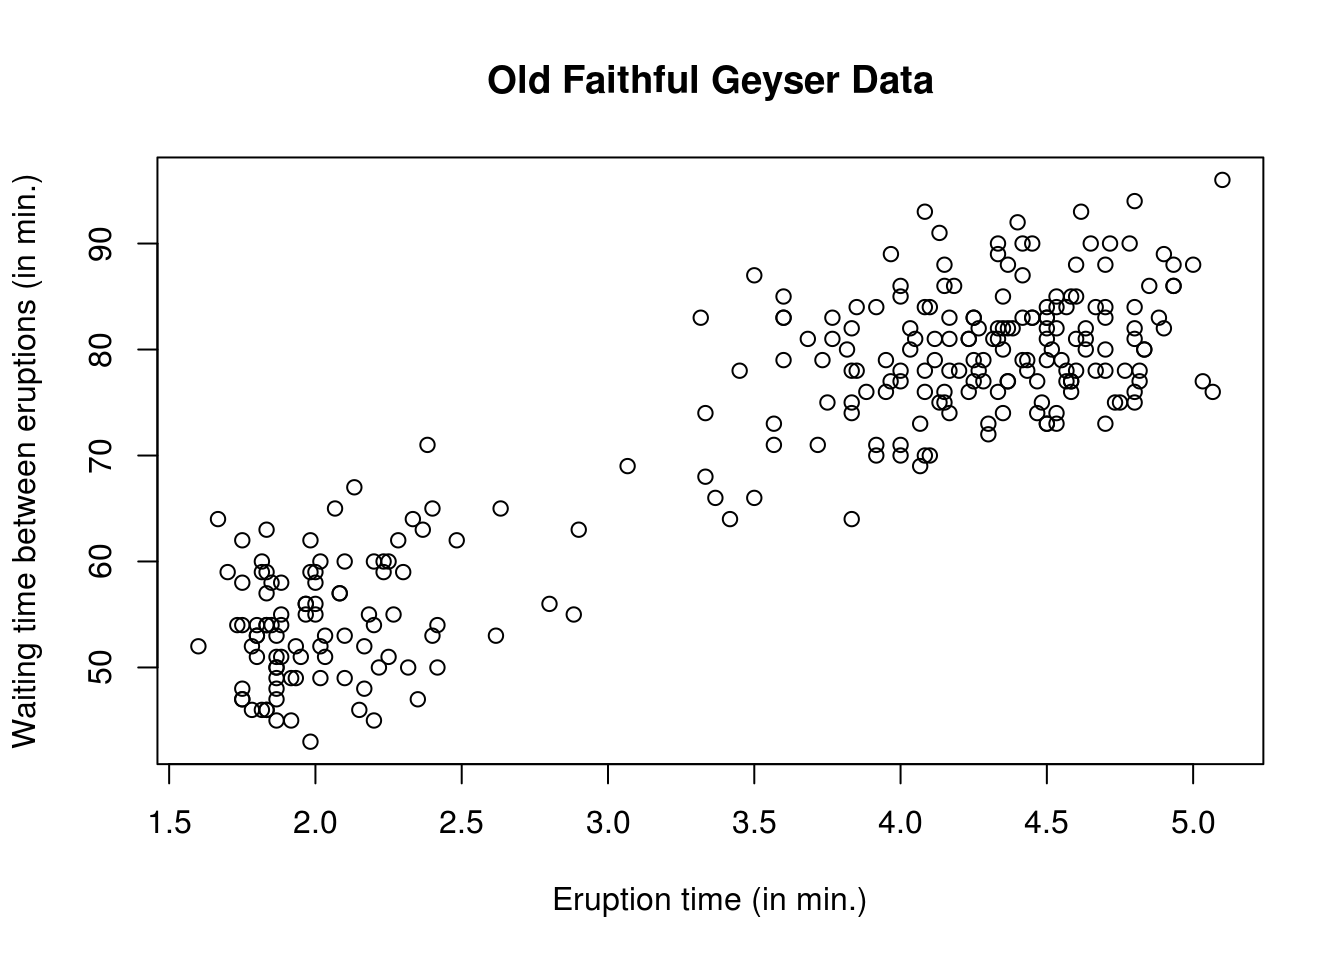
\includegraphics{LinesRModels_files/figure-latex/week1_scatterplot-1.pdf}

\begin{Shaded}
\begin{Highlighting}[]
\CommentTok{#using the grammar of graphics (more modular)}
\CommentTok{#install.packages("ggplot2") #do this once only}
\KeywordTok{library}\NormalTok{(ggplot2)}
\NormalTok{ggplot2}\OperatorTok{::}\KeywordTok{ggplot}\NormalTok{(}\DataTypeTok{data =}\NormalTok{ faithful, }\KeywordTok{aes}\NormalTok{(}\DataTypeTok{x =}\NormalTok{ eruptions, }\DataTypeTok{y =}\NormalTok{ waiting)) }\OperatorTok{+}\StringTok{ }
\StringTok{  }\KeywordTok{geom_point}\NormalTok{() }\OperatorTok{+}\StringTok{  }
\StringTok{  }\KeywordTok{labs}\NormalTok{(}\DataTypeTok{title =} \StringTok{"Old Faithful Geyser Data"}\NormalTok{, }
       \DataTypeTok{x =} \StringTok{"Eruption time (in min.)"}\NormalTok{, }
       \DataTypeTok{y =} \StringTok{"Waiting time between eruptions (in min.)"}\NormalTok{)}
\end{Highlighting}
\end{Shaded}

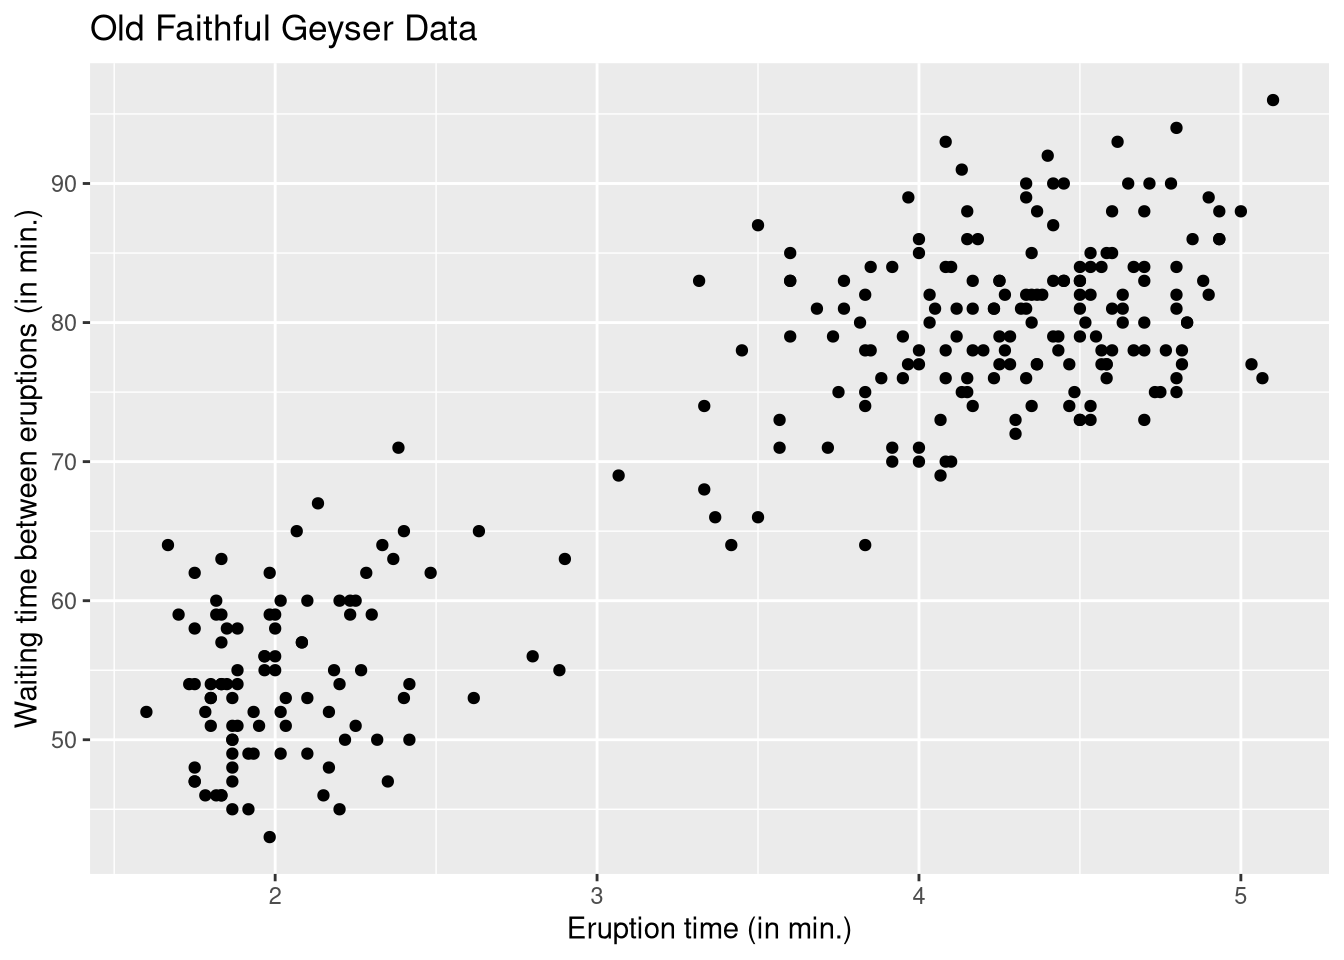
\includegraphics{LinesRModels_files/figure-latex/week1_scatterplot-2.pdf}

A simple linear model of the form
\[y_i = \beta_0 + \beta_1 \mathrm{x}_i + \varepsilon_i,\] where
\(\varepsilon_i\) is a noise variable with expectation zero and
\(\mathbf{x} = \mathsf{eruptions}\) and
\(\boldsymbol{y} = \mathsf{waiting}\). We first create a matrix with a
column of \(\mathbf{1}_n\) for the intercept. We bind vectors by column
(\texttt{cbind}) into a matrix, recycling arguments if necessary. Use
\texttt{\$} to obtain a column of the data frame based on the name of
the variable (partial matching is allowed, e.g., \texttt{faithful\$er}
is equivalent to \texttt{faithful\$eruptions} in this case).

\begin{Shaded}
\begin{Highlighting}[]
\CommentTok{## Manipulating matrices}
\NormalTok{n <-}\StringTok{ }\KeywordTok{nrow}\NormalTok{(faithful)}
\NormalTok{p <-}\StringTok{ }\KeywordTok{ncol}\NormalTok{(faithful)}
\NormalTok{y <-}\StringTok{ }\NormalTok{faithful}\OperatorTok{$}\NormalTok{waiting}
\NormalTok{X <-}\StringTok{ }\KeywordTok{cbind}\NormalTok{(}\DecValTok{1}\NormalTok{, faithful}\OperatorTok{$}\NormalTok{eruptions)}
\end{Highlighting}
\end{Shaded}

\hypertarget{projection-matrices}{%
\subsection{Projection matrices}\label{projection-matrices}}

Recall that
\(\mathbf{H}_{\mathbf{X}} \equiv \mathbf{X}(\mathbf{X}^\top\mathbf{X})^{-1}\mathbf{X}^\top\)
is the orthogonal projection matrix onto \(\mathsf{span}(\mathbf{X})\).
The latter has \(p=2\) eigenvalues equal to 1, is an \(n \times n\)
matrix of rank \(p\), is symmetric and idempotent. We can verify the
properties of \(\mathbf{H}_{\mathbf{X}}\) numerically.

\BeginKnitrBlock{rmdcaution}
Whereas we will frequently use \texttt{==} to check for equality of
booleans, the latter should be avoided for comparisons because computer
arithmetic is exact only in base 2. For example,
\texttt{1/10\ +\ 2/10\ -\ 3/10\ ==\ 0} will return \texttt{FALSE},
whereas \texttt{all.equal(1/10\ +\ 2/10\ -\ 3/10,\ 0)} will return
\texttt{TRUE}. Use \texttt{all.equal} to check for equalities.
\EndKnitrBlock{rmdcaution}

\begin{Shaded}
\begin{Highlighting}[]
\NormalTok{Hx <-}\StringTok{ }\NormalTok{X }\OperatorTok\StringTok{ }\KeywordTok{solve}\NormalTok{(}\KeywordTok{crossprod}\NormalTok{(X)) }\OperatorTok\StringTok{ }\KeywordTok{t}\NormalTok{(X)}
\CommentTok{# Create projection matrix onto complement }
\CommentTok{# `diag(n)` is the n by n identity matrix}
\NormalTok{Mx <-}\StringTok{ }\KeywordTok{diag}\NormalTok{(n) }\OperatorTok{-}\StringTok{ }\NormalTok{Hx}
\CommentTok{#Check that projection leaves X invariant}
\KeywordTok{isTRUE}\NormalTok{(}\KeywordTok{all.equal}\NormalTok{(X, Hx }\OperatorTok\StringTok{ }\NormalTok{X))}
\end{Highlighting}
\end{Shaded}

\begin{verbatim}
## [1] TRUE
\end{verbatim}

\begin{Shaded}
\begin{Highlighting}[]
\CommentTok{#Check that orthogonal projection maps X to zero matrix of dimension (n, p)}
\KeywordTok{isTRUE}\NormalTok{(}\KeywordTok{all.equal}\NormalTok{(}\KeywordTok{matrix}\NormalTok{(}\DecValTok{0}\NormalTok{, }\DataTypeTok{nrow =}\NormalTok{ n, }\DataTypeTok{ncol =}\NormalTok{ p), Mx }\OperatorTok\StringTok{ }\NormalTok{X))}
\end{Highlighting}
\end{Shaded}

\begin{verbatim}
## [1] TRUE
\end{verbatim}

\begin{Shaded}
\begin{Highlighting}[]
\CommentTok{#Check that the matrix Hx is idempotent}
\KeywordTok{isTRUE}\NormalTok{(}\KeywordTok{all.equal}\NormalTok{(Hx }\OperatorTok\StringTok{ }\NormalTok{Hx, Hx))}
\end{Highlighting}
\end{Shaded}

\begin{verbatim}
## [1] TRUE
\end{verbatim}

\begin{Shaded}
\begin{Highlighting}[]
\CommentTok{#Check that the matrix Hx is symmetric}
\KeywordTok{isTRUE}\NormalTok{(}\KeywordTok{all.equal}\NormalTok{(}\KeywordTok{t}\NormalTok{(Hx), Hx))}
\end{Highlighting}
\end{Shaded}

\begin{verbatim}
## [1] TRUE
\end{verbatim}

\begin{Shaded}
\begin{Highlighting}[]
\CommentTok{#Check that only a two eigenvalue are 1 and the rest are zero}
\KeywordTok{isTRUE}\NormalTok{(}\KeywordTok{all.equal}\NormalTok{(}\KeywordTok{eigen}\NormalTok{(Hx, }\DataTypeTok{only.values =} \OtherTok{TRUE}\NormalTok{)}\OperatorTok{$}\NormalTok{values, }\KeywordTok{c}\NormalTok{(}\KeywordTok{rep}\NormalTok{(}\DecValTok{1}\NormalTok{, p), }\KeywordTok{rep}\NormalTok{(}\DecValTok{0}\NormalTok{, n }\OperatorTok{-}\StringTok{ }\NormalTok{p))))}
\end{Highlighting}
\end{Shaded}

\begin{verbatim}
## [1] TRUE
\end{verbatim}

\begin{Shaded}
\begin{Highlighting}[]
\CommentTok{#Check that the matrix has rank p}
\KeywordTok{isTRUE}\NormalTok{(}\KeywordTok{all.equal}\NormalTok{(Matrix}\OperatorTok{::}\KeywordTok{rankMatrix}\NormalTok{(Hx), p, }\DataTypeTok{check.attributes =} \OtherTok{FALSE}\NormalTok{))}
\end{Highlighting}
\end{Shaded}

\begin{verbatim}
## [1] TRUE
\end{verbatim}

\hypertarget{exercises}{%
\section{Exercises}\label{exercises}}

\hypertarget{auto-dataset}{%
\subsection{Auto dataset}\label{auto-dataset}}

\begin{itemize}
\tightlist
\item
  Install the \textbf{R} package \texttt{ISLR} and load the dataset
  \texttt{Auto}. Be careful, as \textbf{R} is case-sensitive.
\item
  Query the help file for information about the dataset.
\item
  Look at the first lines of \texttt{Auto}
\item
  Create an explanatory variable \texttt{x} with horsepower and mileage
  per gallon as response \texttt{y}.
\item
  Create a scatterplot of \texttt{y} against \texttt{x}. Is there
  evidence of a linear relationship between the two variables?
\item
  Append a column vector of ones to \texttt{x} and create a projection
  matrix.
\item
  Check that the resulting projection matrix is symmetric and
  idempotent.
\end{itemize}

\hypertarget{oblique-projections-exercise-1.4}{%
\subsection{Oblique projections (exercise
1.4)}\label{oblique-projections-exercise-1.4}}

Suppose that
\(\mathsf{span}(\mathbf{X}) \neq \mathsf{span}(\mathbf{W})\), that both
\(\mathbf{X}\) and \(\mathbf{W}\) are full-rank \(n \times p\) matrices
such that \(\mathbf{X}^\top\mathbf{W}\) and
\(\mathbf{W}^\top\mathbf{X}\) are invertible. An oblique projection
matrix is of the form
\(\mathbf{P}\equiv\mathbf{X}(\mathbf{W}^\top\mathbf{X})^{-1}\mathbf{W}^\top\)
and appears in instrumental variable regression. The oblique projection
is such that \(\mathrm{im}(\mathbf{P})=\mathsf{span}(\mathbf{X})\), but
\(\mathrm{im}(\mathbf{I}-\mathbf{P})=\mathsf{span}(\mathbf{W}^\perp)\).
This fact is illustrated below.

We consider two non-parallel vectors in \(\mathbb{R}^2\), \(\mathbf{X}\)
and \(\mathbf{W}\).

\begin{Shaded}
\begin{Highlighting}[]
\CommentTok{#Create two vectors (non-parallel)}
\NormalTok{x <-}\StringTok{ }\KeywordTok{c}\NormalTok{(}\DecValTok{1}\NormalTok{, }\DecValTok{2}\NormalTok{)}
\NormalTok{w <-}\StringTok{ }\KeywordTok{c}\NormalTok{(}\OperatorTok{-}\DecValTok{1}\NormalTok{, }\FloatTok{0.1}\NormalTok{)}
\CommentTok{#Create oblique projection matrix}
\NormalTok{P <-}\StringTok{ }\NormalTok{x }\OperatorTok\StringTok{ }\KeywordTok{solve}\NormalTok{(}\KeywordTok{t}\NormalTok{(w) }\OperatorTok\StringTok{ }\NormalTok{x) }\OperatorTok\StringTok{ }\KeywordTok{t}\NormalTok{(w)}

\KeywordTok{isTRUE}\NormalTok{(}\KeywordTok{all.equal}\NormalTok{((P }\OperatorTok\StringTok{ }\NormalTok{P), P)) }\CommentTok{#P is idempotent}
\end{Highlighting}
\end{Shaded}

\begin{verbatim}
## [1] TRUE
\end{verbatim}

\begin{Shaded}
\begin{Highlighting}[]
\NormalTok{P }\OperatorTok{-}\StringTok{ }\KeywordTok{t}\NormalTok{(P) }\CommentTok{#but not symmetric}
\end{Highlighting}
\end{Shaded}

\begin{verbatim}
##       [,1]   [,2]
## [1,] 0.000 -2.625
## [2,] 2.625  0.000
\end{verbatim}

The figure below shows the projection of a third vector \(\mathbf{v}\)
(non-parallel to \(\mathbf{X}\) or \(\mathbf{W}\)) onto the span of
{\(\mathbf{P}\) (blue)}, {\(\mathbf{P}^\top\) (red)},
{\(\mathbf{I}_2-\mathbf{P}\) (dashed cyan)} and
{\(\mathbf{I}_2-\mathbf{P}^\top\) (dashed orange)}. The circles indicate
the vectors {\(\mathbf{W}\) (red)} and {\(\mathbf{X}\) (blue)} on the
plane. Notice that \(\mathbf{I}_2-\mathbf{P}^\top \perp \mathbf{P}\),
whereas \(\mathbf{I}_2-\mathbf{P} \perp \mathbf{P}^\top\).

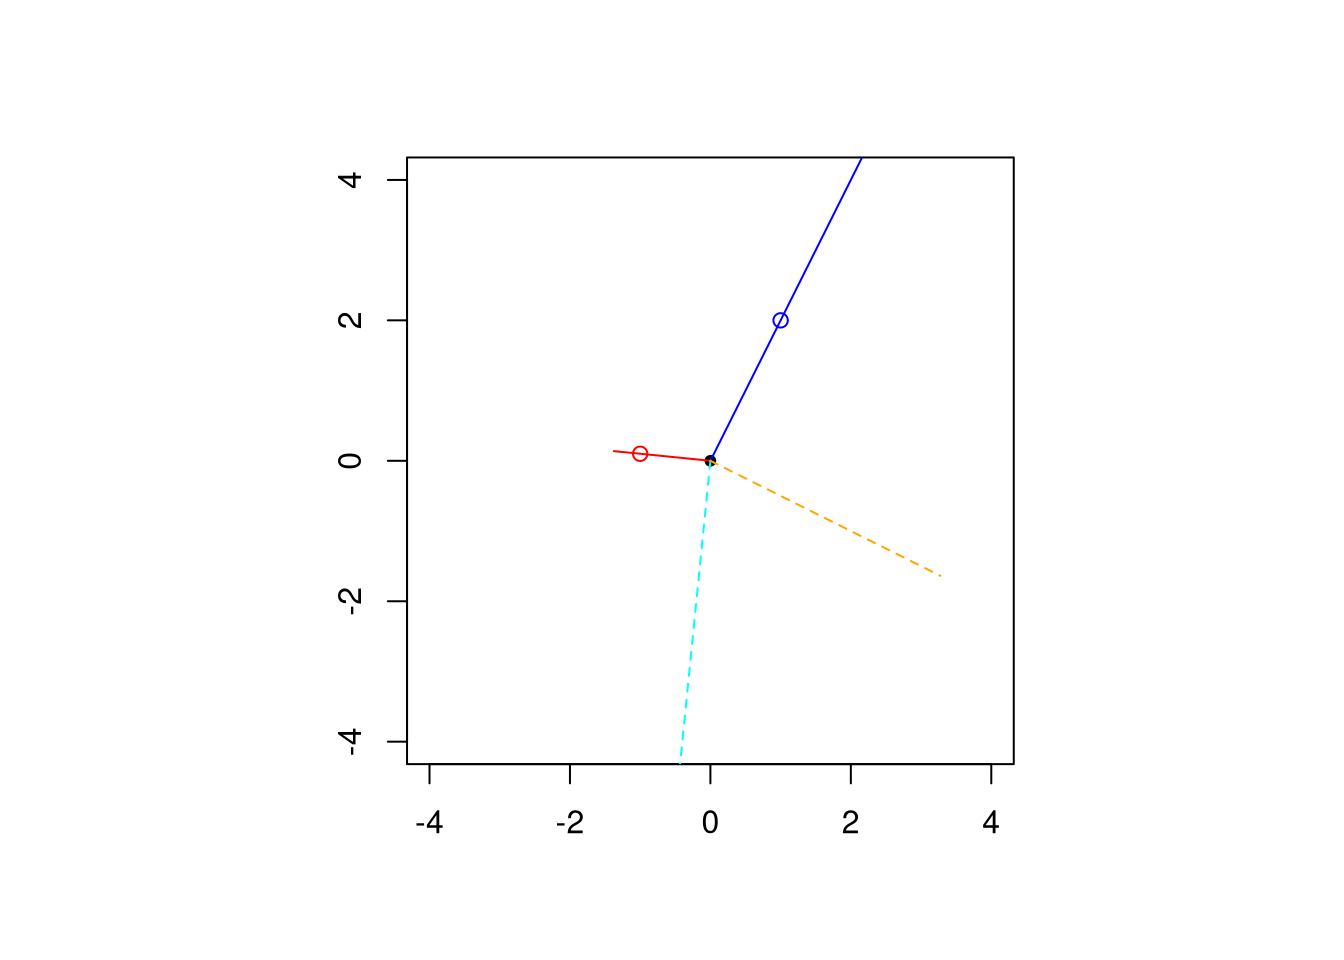
\includegraphics{LinesRModels_files/figure-latex/illustproj-1.pdf}

\hypertarget{summary-of-week-1}{%
\section{Summary of week 1}\label{summary-of-week-1}}

Let \(\mathbf{X}\) be an \(n \times p\) full-rank matrix (\(p <n\)). An
\(n \times n\) orthogonal projection matrix \(\mathbf{H}\)

\begin{itemize}
\tightlist
\item
  projects on to \(\mathcal{V} \subseteq \mathbb{R}^n\), meaning
  \(\mathbf{Hv} \in \mathcal{V}\) for any
  \(\mathbf{v} \in \mathbb{R}^n\);
\item
  is idempotent, meaning \(\mathbf{H} = \mathbf{HH}\);
\item
  is symmetric, meaning \(\mathbf{H} = \mathbf{H}^\top\).
\end{itemize}

The projection matrix \(\mathbf{H}\) is unique; if
\(\mathcal{V} = \mathsf{span}(\mathbf{X})\), then
\[\mathbf{H}_{\mathbf{X}} = \mathbf{X}(\mathbf{X}^\top\mathbf{X})^{-1}\mathbf{X}^\top.\]
Since \(\mathbf{X}: \mathbb{R}^n \to \mathbb{R}^p\),
\(\mathbf{H}_{\mathbf{X}}\) has rank \(p\). The orthogonal complement
\(\mathbf{M}_{\mathbf{X}}\equiv \mathbf{I}_n - \mathbf{H}_{\mathbf{X}}\)
projects onto \(\mathsf{span}^{\perp}(\mathbf{X})\).

\hypertarget{computational-considerations}{%
\chapter{Computational
considerations}\label{computational-considerations}}

In this tutorial, we will explore some basic \textbf{R} commands and
illustrate their use on the Auto dataset (\texttt{Auto}) from the
\texttt{ISLR} package.

\hypertarget{calculation-of-least-square-estimates}{%
\section{Calculation of least square
estimates}\label{calculation-of-least-square-estimates}}

Consider as usual \(\boldsymbol{y}\) and \(n\)-vector of response
variables and a full-rank \(n \times p\) design matrix \(\mathbf{X}\).
We are interested in finding the ordinary least square coefficient
\(\hat{\boldsymbol{\beta}}\), the fitted values
\(\hat{\boldsymbol{y}} = \mathbf{X}\hat{\boldsymbol{\beta}}\) and the
residuals
\(\boldsymbol{e} = \boldsymbol{y} - \mathbf{X}\boldsymbol{\beta}\).

Whereas orthogonal projection matrices are useful for theoretical
derivations, they are not used for computations. Building
\(\mathbf{H}_{\mathbf{X}}\) involves a matrix inversion and the storage
of an \(n \times n\) matrix. In Exercise series 2, we looked at two
matrix decompositions: a singular value decomposition (SVD) and a QR
decomposition. These are more numerically stable than using the normal
equations
\((\mathbf{X}^\top\mathbf{X})\boldsymbol{\beta} = \mathbf{X}^\top\boldsymbol{y}\)
(the condition number of the matrix \(\mathbf{X}^\top\mathbf{X}\) is the
square of that of \(\mathbf{X}\) --- more on this later).

\emph{Optional material}: for more details about the complexity and
algorithms underlying the different methods, the reader is referred to
these notes of
\href{www.math.uchicago.edu/~may/REU2012/REUPapers/Lee.pdf}{Lee}.

\hypertarget{normal-equations}{%
\subsection{Normal equations}\label{normal-equations}}

The following simply illustrates what has been derived in Exercise
series 2. You will probably never use these commands, as \textbf{R} has
devoted functions that are coded more efficiently. We can compute first
the ordinary least square estimates using the formula
\(\hat{\boldsymbol{\beta}} = (\mathbf{X}^\top\mathbf{X})^{-1}\mathbf{X}^\top\boldsymbol{y}\).

\begin{Shaded}
\begin{Highlighting}[]
\KeywordTok{data}\NormalTok{(Auto, }\DataTypeTok{package =} \StringTok{"ISLR"}\NormalTok{)}
\NormalTok{y <-}\StringTok{ }\NormalTok{Auto}\OperatorTok{$}\NormalTok{mpg}
\NormalTok{X <-}\StringTok{ }\KeywordTok{cbind}\NormalTok{(}\DecValTok{1}\NormalTok{, Auto}\OperatorTok{$}\NormalTok{horsepower)}
\NormalTok{n <-}\StringTok{ }\KeywordTok{nrow}\NormalTok{(X)}
\NormalTok{p <-}\StringTok{ }\KeywordTok{ncol}\NormalTok{(X)}
\CommentTok{# Estimation of betahat:}
\NormalTok{XtX <-}\StringTok{ }\KeywordTok{crossprod}\NormalTok{(X)}
\NormalTok{Xty <-}\StringTok{ }\KeywordTok{crossprod}\NormalTok{(X, y)}
\CommentTok{# Solve normal equations}
\NormalTok{betahat <-}\StringTok{ }\KeywordTok{as.vector}\NormalTok{(}\KeywordTok{solve}\NormalTok{(XtX, Xty))}
\CommentTok{#same as betahat <- solve(t(X) %*% X) %*% t(X) %*% y}
\end{Highlighting}
\end{Shaded}

\hypertarget{singular-value-decomposition}{%
\subsection{Singular value
decomposition}\label{singular-value-decomposition}}

The SVD decomposition in \textbf{R} returns a list with elements
\texttt{u}, \texttt{d} and \texttt{v}. \texttt{u} is the orthonormal
\(n \times p\) matrix, \texttt{d} is a vector containing the diagonal
elements of \(\mathbf{D}\) and \texttt{v} is the \(p \times p\)
orthogonal matrix. Recall that the decomposition is
\[\mathbf{X} = \mathbf{UDV}^\top\] and that
\(\mathbf{VV}^\top= \mathbf{V}^\top\mathbf{V}=\mathbf{U}^\top\mathbf{U}=\mathbf{I}_p\).
The matrix \(\mathbf{D}\) contains the singular values of
\(\mathbf{X}\), and the diagonal elements \(\mathrm{d}_{ii}^2\)
corresponds to the (ordered) eigenvalues of
\(\mathbf{X}^\top\mathbf{X}\).

\begin{Shaded}
\begin{Highlighting}[]
\NormalTok{svdX <-}\StringTok{ }\KeywordTok{svd}\NormalTok{(X)}
\CommentTok{# Projection matrix}
\NormalTok{Hx <-}\StringTok{ }\KeywordTok{tcrossprod}\NormalTok{(svdX}\OperatorTok{$}\NormalTok{u)}
\CommentTok{# t(U) %*% U gives p by p identity matrix}
\KeywordTok{all.equal}\NormalTok{(}\KeywordTok{crossprod}\NormalTok{(svdX}\OperatorTok{$}\NormalTok{u), }\KeywordTok{diag}\NormalTok{(p))}
\end{Highlighting}
\end{Shaded}

\begin{verbatim}
## [1] TRUE
\end{verbatim}

\begin{Shaded}
\begin{Highlighting}[]
\CommentTok{# V is an orthogonal matrix}
\KeywordTok{all.equal}\NormalTok{(}\KeywordTok{tcrossprod}\NormalTok{(svdX}\OperatorTok{$}\NormalTok{v), }\KeywordTok{diag}\NormalTok{(p))}
\end{Highlighting}
\end{Shaded}

\begin{verbatim}
## [1] TRUE
\end{verbatim}

\begin{Shaded}
\begin{Highlighting}[]
\KeywordTok{all.equal}\NormalTok{(}\KeywordTok{crossprod}\NormalTok{(svdX}\OperatorTok{$}\NormalTok{v), }\KeywordTok{diag}\NormalTok{(p))}
\end{Highlighting}
\end{Shaded}

\begin{verbatim}
## [1] TRUE
\end{verbatim}

\begin{Shaded}
\begin{Highlighting}[]
\CommentTok{# D contains singular values}
\KeywordTok{all.equal}\NormalTok{(svdX}\OperatorTok{$}\NormalTok{d}\OperatorTok{^}\DecValTok{2}\NormalTok{, }\KeywordTok{eigen}\NormalTok{(XtX, }\DataTypeTok{only.values =} \OtherTok{TRUE}\NormalTok{)}\OperatorTok{$}\NormalTok{values)}
\end{Highlighting}
\end{Shaded}

\begin{verbatim}
## [1] TRUE
\end{verbatim}

\begin{Shaded}
\begin{Highlighting}[]
\CommentTok{# OLS coefficient from SVD}
\NormalTok{betahat_svd <-}\StringTok{ }\KeywordTok{c}\NormalTok{(svdX}\OperatorTok{$}\NormalTok{v }\OperatorTok\StringTok{  }\KeywordTok{diag}\NormalTok{(}\DecValTok{1}\OperatorTok{/}\NormalTok{svdX}\OperatorTok{$}\NormalTok{d) }\OperatorTok\StringTok{ }\KeywordTok{t}\NormalTok{(svdX}\OperatorTok{$}\NormalTok{u) }\OperatorTok\StringTok{ }\NormalTok{y)}
\KeywordTok{all.equal}\NormalTok{(betahat_svd, betahat)}
\end{Highlighting}
\end{Shaded}

\begin{verbatim}
## [1] TRUE
\end{verbatim}

\hypertarget{qr-decomposition}{%
\subsection{QR decomposition}\label{qr-decomposition}}

\textbf{R} uses a QR-decomposition to calculate the OLS. There are
specific functions to return coefficients, fitted values and residuals.
One can also obtain the \(n \times p\) matrix \(\mathbf{Q}_1\) and the
upper triangular \(p \times p\) matrix \(\mathbf{R}\) from the thinned
QR decomposition, \[\mathbf{X} = \mathbf{Q}_1\mathbf{R}.\]

\begin{Shaded}
\begin{Highlighting}[]
\NormalTok{qrX <-}\StringTok{ }\KeywordTok{qr}\NormalTok{(X)}
\NormalTok{Q1 <-}\StringTok{ }\KeywordTok{qr.Q}\NormalTok{(qrX)}
\NormalTok{R <-}\StringTok{ }\KeywordTok{qr.R}\NormalTok{(qrX)}
\CommentTok{# Compute betahat from QR}
\NormalTok{betahat_qr1 <-}\StringTok{ }\KeywordTok{qr.coef}\NormalTok{(qrX, y) }\CommentTok{#using built-in function}
\NormalTok{betahat_qr2 <-}\StringTok{ }\KeywordTok{c}\NormalTok{(}\KeywordTok{backsolve}\NormalTok{(R, }\KeywordTok{t}\NormalTok{(Q1) }\OperatorTok\StringTok{ }\NormalTok{y)) }\CommentTok{#manually}
\KeywordTok{all.equal}\NormalTok{(betahat, betahat_qr1, }\DataTypeTok{check.attributes =} \OtherTok{FALSE}\NormalTok{)}
\end{Highlighting}
\end{Shaded}

\begin{verbatim}
## [1] TRUE
\end{verbatim}

\begin{Shaded}
\begin{Highlighting}[]
\KeywordTok{all.equal}\NormalTok{(betahat, betahat_qr2, }\DataTypeTok{check.attributes =} \OtherTok{FALSE}\NormalTok{)}
\end{Highlighting}
\end{Shaded}

\begin{verbatim}
## [1] TRUE
\end{verbatim}

\begin{Shaded}
\begin{Highlighting}[]
\CommentTok{# Compute residuals}
\NormalTok{qre <-}\StringTok{ }\KeywordTok{qr.resid}\NormalTok{(qrX, y)}
\KeywordTok{all.equal}\NormalTok{(qre, }\KeywordTok{c}\NormalTok{(y }\OperatorTok{-}\StringTok{ }\NormalTok{X }\OperatorTok\StringTok{ }\NormalTok{betahat), }\DataTypeTok{check.attributes =} \OtherTok{FALSE}\NormalTok{)}
\end{Highlighting}
\end{Shaded}

\begin{verbatim}
## [1] TRUE
\end{verbatim}

\begin{Shaded}
\begin{Highlighting}[]
\CommentTok{# Compute fitted values}
\NormalTok{qryhat <-}\StringTok{ }\KeywordTok{qr.fitted}\NormalTok{(qrX, y)}
\KeywordTok{all.equal}\NormalTok{(qryhat, }\KeywordTok{c}\NormalTok{(X }\OperatorTok\StringTok{ }\NormalTok{betahat), }\DataTypeTok{check.attributes =} \OtherTok{FALSE}\NormalTok{)}
\end{Highlighting}
\end{Shaded}

\begin{verbatim}
## [1] TRUE
\end{verbatim}

\begin{Shaded}
\begin{Highlighting}[]
\CommentTok{# Compute orthogonal projection matrix}
\NormalTok{qrHx <-}\StringTok{ }\KeywordTok{tcrossprod}\NormalTok{(Q1)}
\KeywordTok{all.equal}\NormalTok{(qrHx, Hx)}
\end{Highlighting}
\end{Shaded}

\begin{verbatim}
## [1] TRUE
\end{verbatim}

\hypertarget{parameter-estimation}{%
\section{Parameter estimation}\label{parameter-estimation}}

We are now ready to fit a simple linear model with an intercept and a
linear effect for the weight,
\[ \texttt{mpg}_i = \beta_0 + \texttt{hp}_i\beta_1 +\varepsilon_i.\] We
form the design matrix
\((\boldsymbol{1}_n^\top, \texttt{hp}^\top)^\top\) and the vector of
regressand \(\texttt{mpg}\), then proceed with calculating the OLS
coefficients \(\hat{\boldsymbol{\beta}}\), the hat matrix
\(\mathbf{H}_{\mathbf{X}}\), the fitted values \(\hat{\boldsymbol{y}}\)
and the residuals \(\boldsymbol{e}\).

\begin{Shaded}
\begin{Highlighting}[]
\CommentTok{#Design matrix}
\NormalTok{hp <-}\StringTok{ }\NormalTok{Auto}\OperatorTok{$}\NormalTok{horsepower}
\NormalTok{X <-}\StringTok{ }\KeywordTok{cbind}\NormalTok{(}\DecValTok{1}\NormalTok{, Auto}\OperatorTok{$}\NormalTok{horsepower)}
\NormalTok{mpg <-}\StringTok{ }\NormalTok{Auto}\OperatorTok{$}\NormalTok{mpg}
\CommentTok{#OLS estimates}
\NormalTok{XtXinv <-}\StringTok{ }\KeywordTok{solve}\NormalTok{(}\KeywordTok{crossprod}\NormalTok{(X))}
\NormalTok{beta_hat <-}\StringTok{ }\KeywordTok{c}\NormalTok{(XtXinv }\OperatorTok\StringTok{ }\KeywordTok{t}\NormalTok{(X) }\OperatorTok\StringTok{ }\NormalTok{mpg)}
\CommentTok{#Form orthogonal projection matrix}
\NormalTok{Hmat <-}\StringTok{ }\NormalTok{X }\OperatorTok\StringTok{ }\NormalTok{XtXinv }\OperatorTok\StringTok{ }\KeywordTok{t}\NormalTok{(X)}
\CommentTok{#Create residuals and fitted values}
\NormalTok{fitted <-}\StringTok{ }\NormalTok{Hmat }\OperatorTok\StringTok{ }\NormalTok{mpg}
\NormalTok{res <-}\StringTok{ }\NormalTok{mpg }\OperatorTok{-}\StringTok{ }\NormalTok{fitted}
\NormalTok{fitted <-}\StringTok{ }\NormalTok{Hmat }\OperatorTok\StringTok{ }\NormalTok{mpg}
\end{Highlighting}
\end{Shaded}

The residuals \(\boldsymbol{e} = \boldsymbol{y} -\hat{\boldsymbol{y}}\)
can be interpreted as the \emph{vertical} distance between the
regression slope and the observation. For each observation \(y_i\), a
vertical line at distance \(e_i\) is drawn from the prediction
\(\hat{y}_i\).

\begin{Shaded}
\begin{Highlighting}[]
\KeywordTok{plot}\NormalTok{(mpg }\OperatorTok{~}\StringTok{ }\NormalTok{horsepower,  }\DataTypeTok{data =}\NormalTok{ Auto, }
     \DataTypeTok{xlab =} \StringTok{"Power of engine (hp)"}\NormalTok{, }
     \DataTypeTok{ylab =} \StringTok{"Fuel economy (miles/US gallon)"}\NormalTok{, }
     \DataTypeTok{main =} \StringTok{"Fuel economy of automobiles"}\NormalTok{,}
     \CommentTok{# the subsequent commands for `plot`  tweak the display}
     \CommentTok{# check for yourself the effect of removing them}
     \CommentTok{# bty = "l" gives L shaped graphical windows (not boxed)}
     \CommentTok{# pch = 20 gives full dots rather than empty circles for points}
     \DataTypeTok{bty =} \StringTok{"l"}\NormalTok{, }\DataTypeTok{pch =} \DecValTok{20}\NormalTok{) }
\CommentTok{#Line of best linear fit}
\KeywordTok{abline}\NormalTok{(}\DataTypeTok{a =}\NormalTok{ beta_hat[}\DecValTok{1}\NormalTok{], }\DataTypeTok{b =}\NormalTok{ beta_hat[}\DecValTok{2}\NormalTok{])}

\CommentTok{#Residuals are vertical distance from line to }
\ControlFlowTok{for}\NormalTok{(i }\ControlFlowTok{in} \DecValTok{1}\OperatorTok{:}\KeywordTok{nrow}\NormalTok{(X))\{}
  \KeywordTok{segments}\NormalTok{(}\DataTypeTok{x0 =}\NormalTok{ hp[i], }\DataTypeTok{y0 =}\NormalTok{ fitted[i], }\DataTypeTok{y1 =}\NormalTok{ fitted[i] }\OperatorTok{+}\StringTok{ }\NormalTok{res[i], }\DataTypeTok{col =} \DecValTok{2}\NormalTok{)}
\NormalTok{\}}
\end{Highlighting}
\end{Shaded}

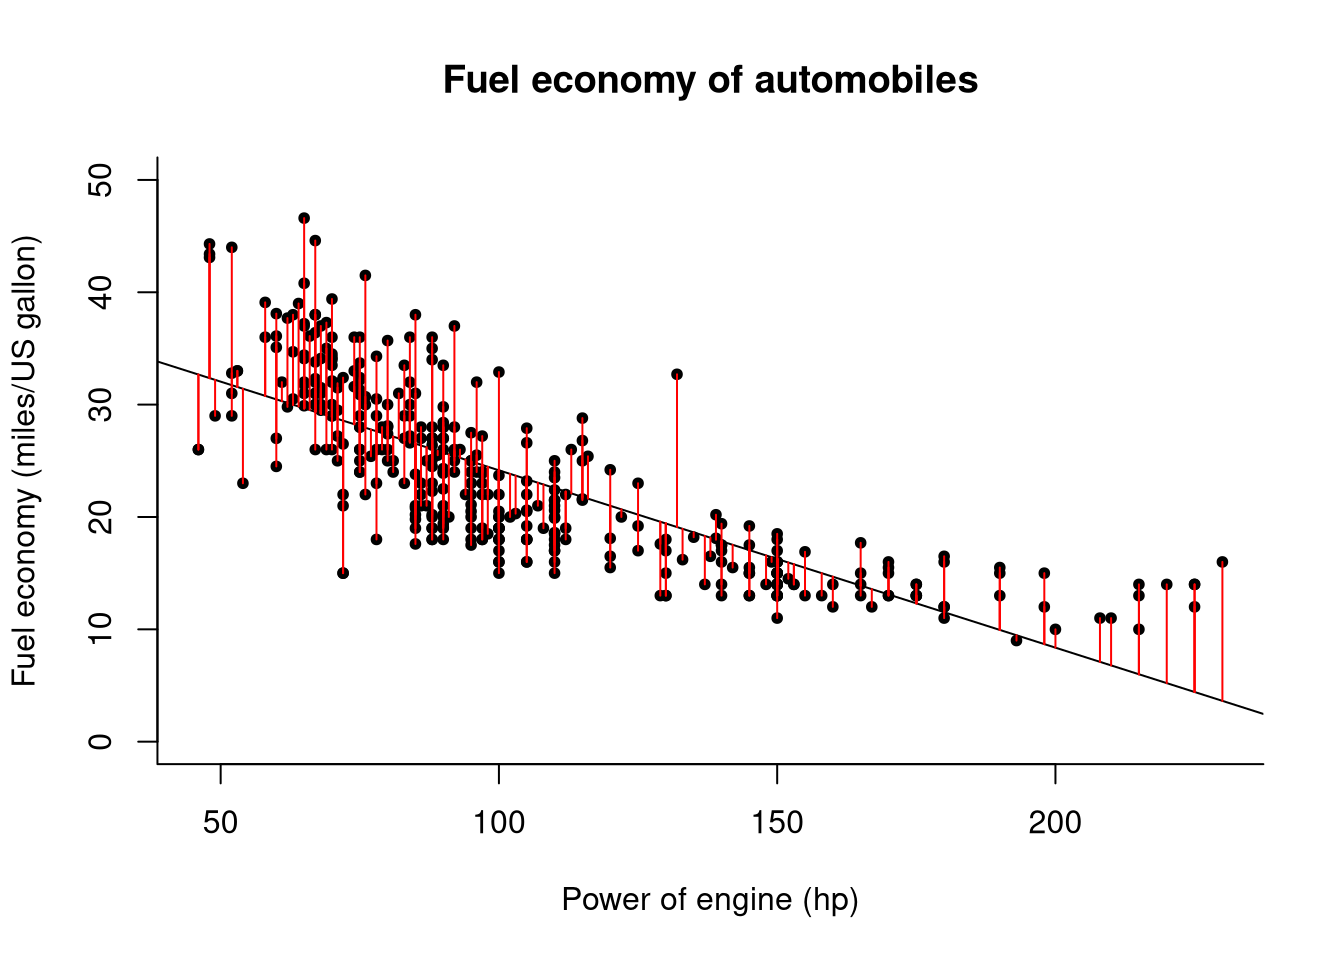
\includegraphics{LinesRModels_files/figure-latex/verticaldist-1.pdf}

The same scatterplot, this time using \texttt{ggplot2}.

\begin{Shaded}
\begin{Highlighting}[]
\KeywordTok{library}\NormalTok{(ggplot2, }\DataTypeTok{warn.conflicts =} \OtherTok{FALSE}\NormalTok{, }\DataTypeTok{quietly =} \OtherTok{TRUE}\NormalTok{)}
\CommentTok{#Create data frame with segments}
\NormalTok{vlines <-}\StringTok{ }\KeywordTok{data.frame}\NormalTok{(}\DataTypeTok{x1 =}\NormalTok{ hp, }\DataTypeTok{y1 =}\NormalTok{ fitted, }\DataTypeTok{y2 =}\NormalTok{ fitted }\OperatorTok{+}\StringTok{ }\NormalTok{res)}
\NormalTok{ggg <-}\StringTok{ }\KeywordTok{ggplot}\NormalTok{(Auto, }\KeywordTok{aes}\NormalTok{(}\DataTypeTok{x =}\NormalTok{ horsepower, }\DataTypeTok{y =}\NormalTok{ mpg)) }\OperatorTok{+}\StringTok{ }
\StringTok{        }\KeywordTok{geom_point}\NormalTok{() }\OperatorTok{+}\StringTok{ }
\StringTok{        }\KeywordTok{labs}\NormalTok{(}\DataTypeTok{x =} \StringTok{"Power of engine (hp)"}\NormalTok{, }
             \DataTypeTok{y =} \StringTok{"Fuel economy (miles/US gallon)"}\NormalTok{, }
             \DataTypeTok{title =} \StringTok{"Fuel economy of automobiles"}\NormalTok{) }\OperatorTok{+}
\StringTok{      }\KeywordTok{geom_segment}\NormalTok{(}\KeywordTok{aes}\NormalTok{(}\DataTypeTok{x =}\NormalTok{ x1, }\DataTypeTok{y =}\NormalTok{ y1, }\DataTypeTok{xend =}\NormalTok{ x1, }\DataTypeTok{yend =}\NormalTok{ y2, }\DataTypeTok{color =} \StringTok{"red"}\NormalTok{), }
                   \DataTypeTok{data =}\NormalTok{ vlines, }\DataTypeTok{show.legend =} \OtherTok{FALSE}\NormalTok{) }\OperatorTok{+}\StringTok{ }
\StringTok{      }\KeywordTok{geom_abline}\NormalTok{(}\DataTypeTok{slope =}\NormalTok{ beta_hat[}\DecValTok{2}\NormalTok{], }\DataTypeTok{intercept =}\NormalTok{ beta_hat[}\DecValTok{1}\NormalTok{])}
\KeywordTok{print}\NormalTok{(ggg)}
\end{Highlighting}
\end{Shaded}

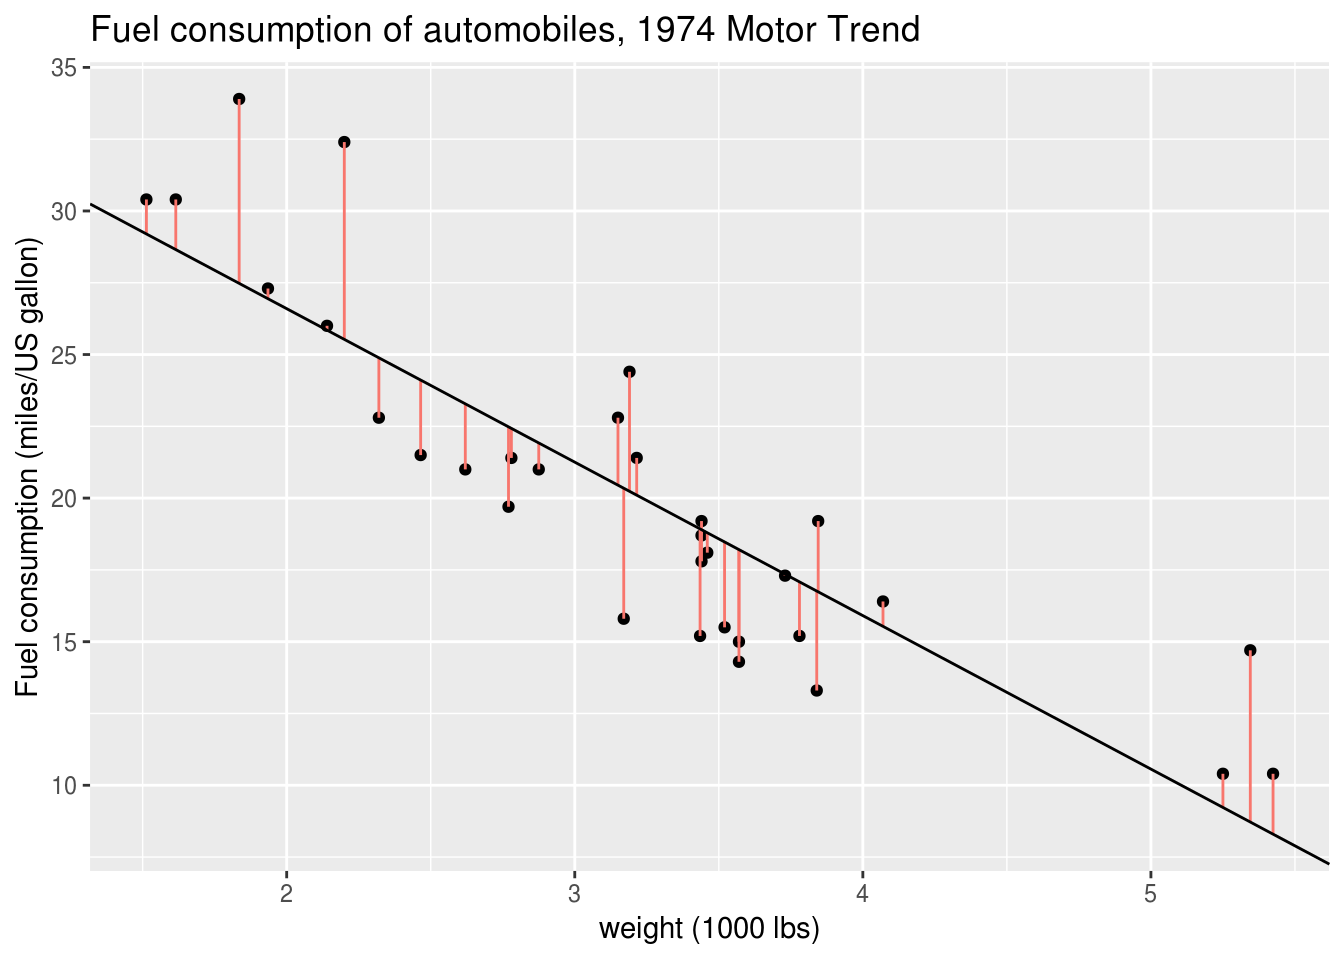
\includegraphics{LinesRModels_files/figure-latex/ggplotmtcars-1.pdf}

\hypertarget{interpretation-of-the-coefficients}{%
\section{Interpretation of the
coefficients}\label{interpretation-of-the-coefficients}}

If the regression model is
\[y_i = \beta_0 + \mathrm{x}_{i1}\beta_1 + \mathrm{x}_{i2}\beta_2 + \varepsilon_i,\]
the interpretation of \(\beta_1\) in the linear model is as follows: a
unit increase in \(x\) leads to \(\beta_1\) units increase in \(y\),
everything else (i.e., \(\mathrm{x}_{i2}\)) being held constant.

For the \texttt{Auto} regression above, an increase of the power of the
engine by one horsepower leads to an average decrease of 0.16 miles per
US gallon in distance covered by the car. We could easily get an
equivalent statement in terms of increase of the car fuel consumption
for a given distance.

\hypertarget{the-lm-function}{%
\section{\texorpdfstring{The \texttt{lm}
function}{The lm function}}\label{the-lm-function}}

The function \texttt{lm} is the workshorse for fitting linear models. It
takes as input a formula: suppose you have a data frame containing
columns \texttt{x} (a regressor) and \texttt{y} (the regressand); you
can then call \texttt{lm(y\ \textasciitilde{}\ x)} to fit the linear
model \(y = \beta_0 + \beta_1x + \varepsilon\). The explanatory variable
\texttt{y} is on the left hand side, while the right hand side should
contain the predictors, separated by a \texttt{+} sign if there are more
than one. If you provide the data frame name using \texttt{data}, then
the shorthand \texttt{y\ \textasciitilde{}\ .} fits all the columns of
the data frame (but \texttt{y}) as regressors.

To fit higher order polynomials or transformations, use the \texttt{I}
function to tell \textbf{R} to interpret the input ``as is''. Thus,
\texttt{lm(y\textasciitilde{}x+I(x\^{}2))}, would fit a linear model
with design matrix
\((\boldsymbol{1}_n, \mathbf{x}^\top, \mathbf{x}^2)^\top\). A constant
is automatically included in the regression, but can be removed by
writing \texttt{-1} or \texttt{+0} on the right hand side of the
formula.

\begin{Shaded}
\begin{Highlighting}[]
\CommentTok{# The function lm and its output}
\NormalTok{fit <-}\StringTok{ }\KeywordTok{lm}\NormalTok{(mpg }\OperatorTok{~}\StringTok{ }\NormalTok{horsepower }\OperatorTok{+}\StringTok{ }\KeywordTok{I}\NormalTok{(horsepower}\OperatorTok{^}\DecValTok{2}\NormalTok{), }\DataTypeTok{data =}\NormalTok{ Auto)}
\NormalTok{fit_summary <-}\StringTok{ }\KeywordTok{summary}\NormalTok{(fit)}
\end{Highlighting}
\end{Shaded}

The \texttt{lm} output will display OLS estimates along with standard
errors, \(t\) values for the Wald test of the hypothesis
\(\mathrm{H}_0: \beta_i=0\) and the associated \(P\)-values. Other
statistics and information about the sample size, the degrees of
freedom, etc., are given at the bottom of the table.

Many methods allow you to extract specific objects. For example, the
functions \texttt{coef}, \texttt{resid}, \texttt{fitted},
\texttt{model.matrix} will return \(\hat{\boldsymbol{\beta}}\),
\(\boldsymbol{e}\), \(\hat{\boldsymbol{y}}\) and \(\mathbf{X}\),
respectively.

\begin{Shaded}
\begin{Highlighting}[]
\KeywordTok{names}\NormalTok{(fit)}
\end{Highlighting}
\end{Shaded}

\begin{verbatim}
##  [1] "coefficients"  "residuals"     "effects"       "rank"         
##  [5] "fitted.values" "assign"        "qr"            "df.residual"  
##  [9] "xlevels"       "call"          "terms"         "model"
\end{verbatim}

\begin{Shaded}
\begin{Highlighting}[]
\KeywordTok{names}\NormalTok{(fit_summary)}
\end{Highlighting}
\end{Shaded}

\begin{verbatim}
##  [1] "call"          "terms"         "residuals"     "coefficients" 
##  [5] "aliased"       "sigma"         "df"            "r.squared"    
##  [9] "adj.r.squared" "fstatistic"    "cov.unscaled"
\end{verbatim}

\hypertarget{the-hyperplane-of-fitted-values}{%
\section{The hyperplane of fitted
values}\label{the-hyperplane-of-fitted-values}}

In class, we presented a linear model for the \texttt{Auto} dataset of
the form
\[\mathsf{mpg}_i = \beta_0 + \beta_1 \mathsf{hp}_i + \beta_2 \mathsf{hp}_i^2 + \varepsilon_i\]
and claimed this was a linear model. This is indeed true because we can
form the design matrix \([\mathbf{1}_n, \mathsf{hp}, \mathsf{hp}^2]\)
and obtain coefficients \(\hat{\boldsymbol{\beta}}\). The graphical
depiction is counterintuitive.

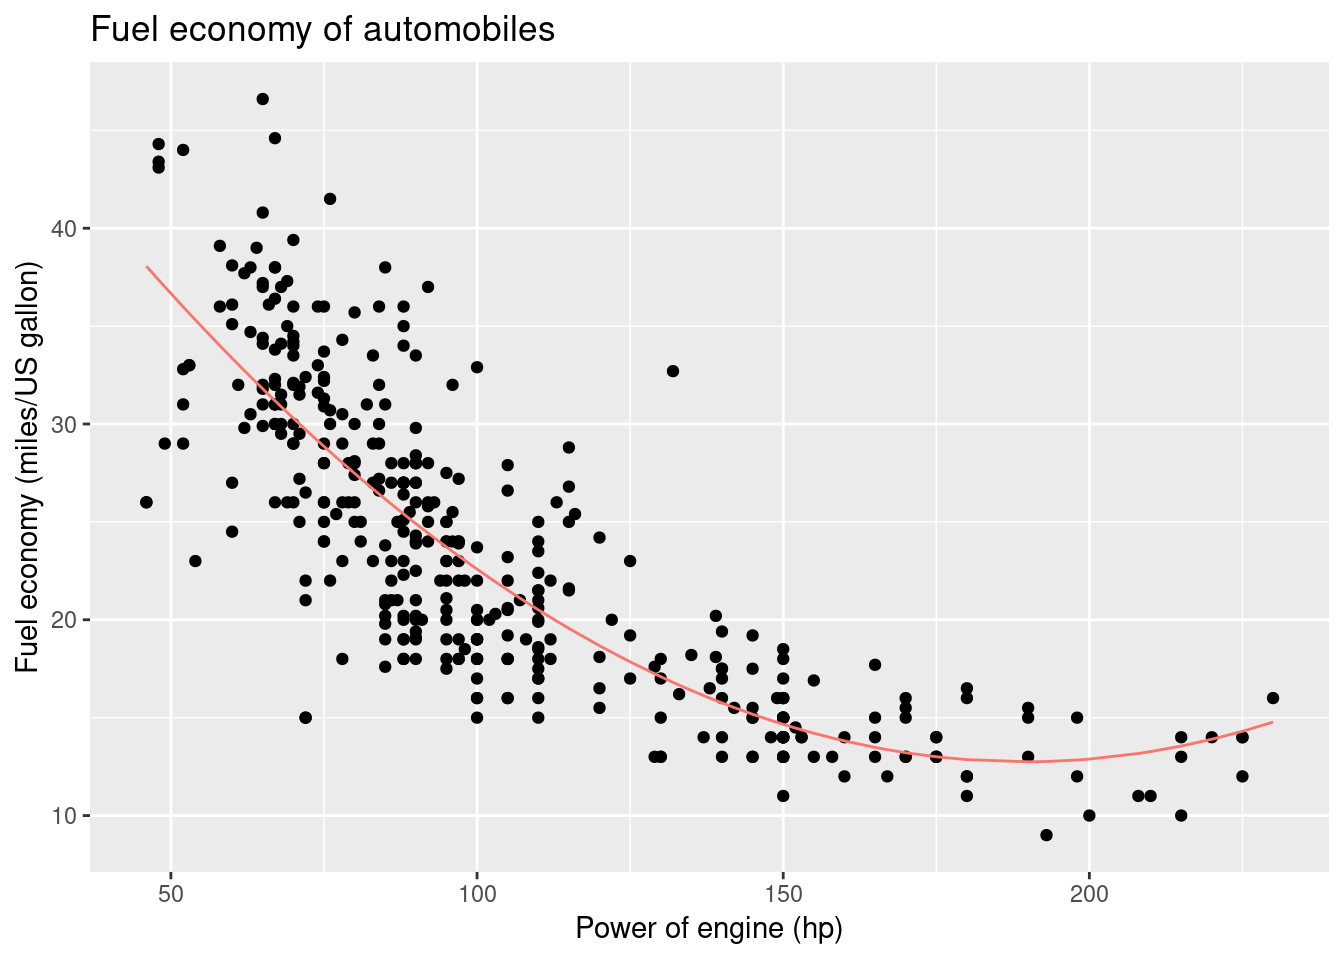
\includegraphics{LinesRModels_files/figure-latex/unnamed-chunk-6-1.pdf}

This quadratic curve is nothing like an hyperplane! Let
\(\boldsymbol{y} \equiv \texttt{mpg}\), \(\mathsf{x} = \texttt{hp}\) and
\(\mathsf{z} = \texttt{hp}^2\). But recall that we are working in three
dimensions (the intercept gives the height of the hyperplane) and the
coordinates of our hyperplane are\\
\[\beta_0 + \beta_1x-y +\beta_2z =0.\] However, the observations will
always be such that \(z = x^2\), so our fitted values will lie on a
one-dimensional subspace of this hyperplane.

The following 3D depiction hopefully captures this better and shows the
fitted hyperplane along with the line on which all the (\(x_i, z_i\))
observations lie.

\begin{verbatim}
## PhantomJS not found. You can install it with webshot::install_phantomjs(). If it is installed, please make sure the phantomjs executable can be found via the PATH variable.
\end{verbatim}

\hypertarget{rgl73574}{}

\hypertarget{centered-coefficient-of-determination}{%
\section{(Centered) coefficient of
determination}\label{centered-coefficient-of-determination}}

Recall the decomposition of observations into fitted and residual
vectors,
\[\boldsymbol{y} = (\boldsymbol{y} - \mathbf{X}\hat{\boldsymbol{\beta}}) + \mathbf{X}\hat{\boldsymbol{\beta}}= \boldsymbol{e} + \hat{\boldsymbol{y}}\]
where
\(\boldsymbol{e} \equiv \mathbf{M}_{\mathbf{X}}\boldsymbol{y} \perp \hat{\boldsymbol{y}} \equiv \mathbf{H}_{\mathbf{X}}\boldsymbol{y}\).

The centered coefficient of determination, \(R^2_c\) measures the
proportion of variation explained by the centered fitted values relative
to the centered observations, i.e.,
\[ R^2_c = \frac{\|\hat{\boldsymbol{y}}-\bar{y}\mathbf{1}_n\|^2}{\|\boldsymbol{y}-\bar{y}\mathbf{1}_n\|^2}=\frac{\|\hat{\boldsymbol{y}}\|^2-\|\bar{y}\mathbf{1}_n\|^2}{\|\boldsymbol{y}\|^2-\|\bar{y}\mathbf{1}_n\|^2}.\]
since the vectors
\(\bar{y}\mathbf{1}_n \perp \hat{\boldsymbol{y}}-\bar{y}\mathbf{1}_n\).

Provided that \(\mathbf{1}_n \in \mathsf{span}(\mathbf{X})\), it is
obvious that the fitted values \(\hat{\boldsymbol{y}}\) are invariant to
linear transformations of the covariates \(\mathbf{X}\). Multiplicative
changes in \(\boldsymbol{y}\) lead to an equivalent change in
\(\boldsymbol{e}\) and \(\hat{\boldsymbol{y}}\). However,
location-changes in \(\boldsymbol{y}\) are only reflected in
\(\hat{\boldsymbol{y}}\) (they are absorbed by the intercept). This is
why \(R^2\) is not invariant to location-changes in the response, since
the ratio \(\|\hat{\boldsymbol{y}}\|^2/\|\boldsymbol{y}\|^2\) increases
to 1 if \({\boldsymbol{y}}\mapsto {\boldsymbol{y}}+ a \mathbf{1}_n\).

This invariance is precisely the reason we dismissed \(R^2\). For
example, a change of units from Farenheit to Celcius, viz.
\(T_c = 5 (T_F - 32)/9\), leads to different values of \(R^2\):

\begin{Shaded}
\begin{Highlighting}[]
\KeywordTok{data}\NormalTok{(aatemp, }\DataTypeTok{package =} \StringTok{"faraway"}\NormalTok{)}
\KeywordTok{plot}\NormalTok{(temp }\OperatorTok{~}\StringTok{ }\NormalTok{year, }\DataTypeTok{data =}\NormalTok{ aatemp, }\DataTypeTok{ylab =} \StringTok{"Temperature (in F)"}\NormalTok{, }\DataTypeTok{bty =} \StringTok{"l"}\NormalTok{)}
\CommentTok{#Form design matrix and two response vectors}
\NormalTok{yF <-}\StringTok{ }\NormalTok{aatemp}\OperatorTok{$}\NormalTok{temp}
\NormalTok{n <-}\StringTok{ }\KeywordTok{length}\NormalTok{(yF)}
\NormalTok{yC <-}\StringTok{ }\DecValTok{5}\OperatorTok{/}\DecValTok{9}\OperatorTok{*}\NormalTok{(aatemp}\OperatorTok{$}\NormalTok{temp }\OperatorTok{-}\StringTok{ }\DecValTok{32}\NormalTok{)}
\NormalTok{X <-}\StringTok{ }\KeywordTok{cbind}\NormalTok{(}\DecValTok{1}\NormalTok{, aatemp}\OperatorTok{$}\NormalTok{year)}
\CommentTok{# Obtain OLS coefficients and fitted values}
\NormalTok{XtX <-}\StringTok{ }\KeywordTok{solve}\NormalTok{(}\KeywordTok{crossprod}\NormalTok{(X))}
\NormalTok{beta_hat_F <-}\StringTok{ }\NormalTok{XtX }\OperatorTok\StringTok{ }\KeywordTok{crossprod}\NormalTok{(X, yF)}
\KeywordTok{abline}\NormalTok{(}\DataTypeTok{a =}\NormalTok{ beta_hat_F[}\DecValTok{1}\NormalTok{], }\DataTypeTok{b =}\NormalTok{ beta_hat_F[}\DecValTok{2}\NormalTok{])}
\end{Highlighting}
\end{Shaded}

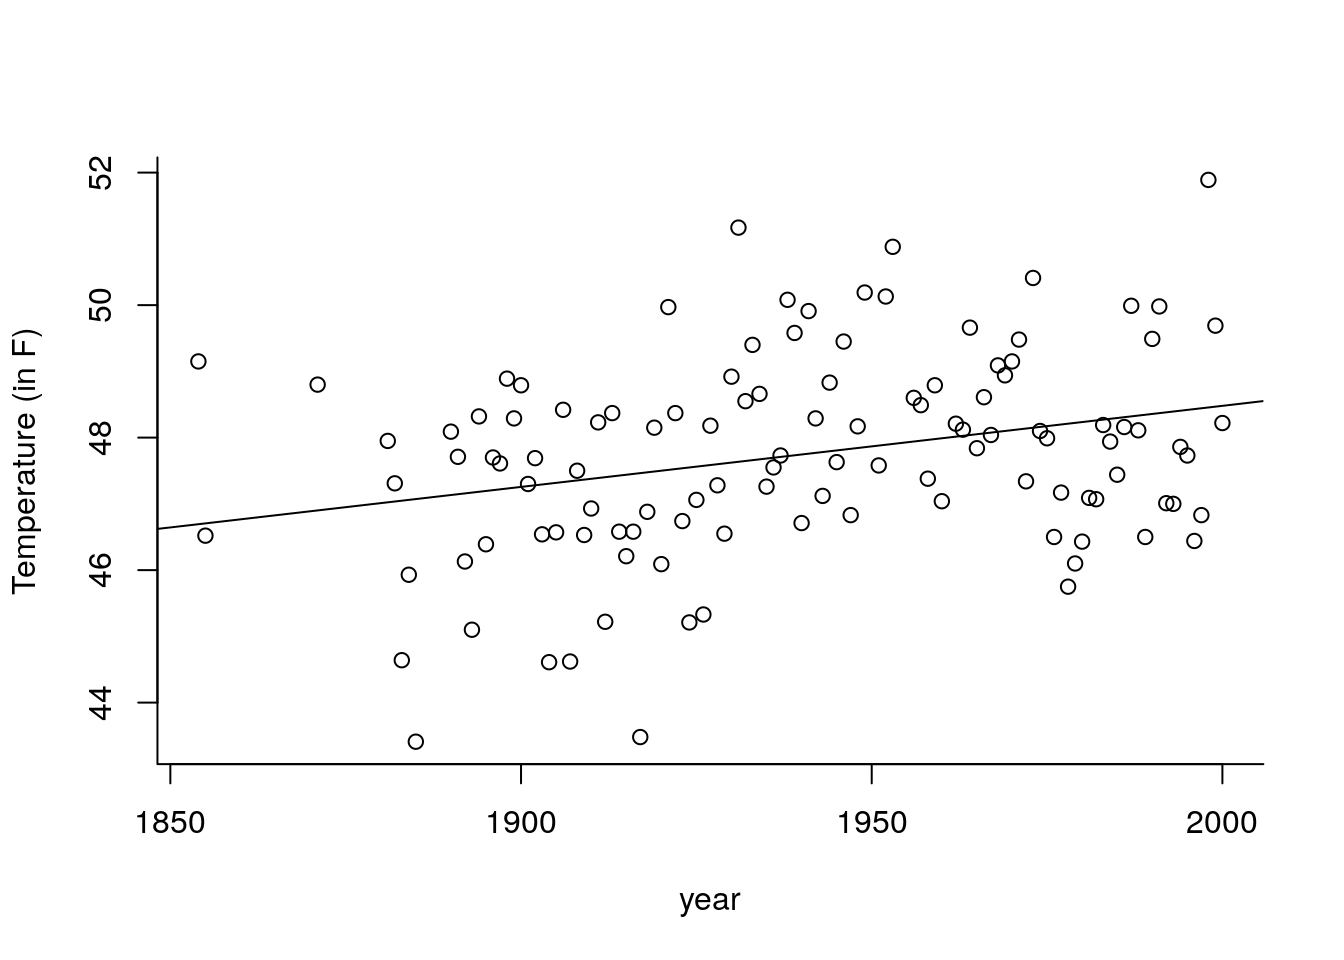
\includegraphics{LinesRModels_files/figure-latex/faraway-1.pdf}

\begin{Shaded}
\begin{Highlighting}[]
\NormalTok{beta_hat_C <-}\StringTok{ }\NormalTok{XtX }\OperatorTok\StringTok{ }\KeywordTok{crossprod}\NormalTok{(X, yC)}
\NormalTok{fitted_F <-}\StringTok{ }\NormalTok{X }\OperatorTok\StringTok{ }\NormalTok{beta_hat_F}
\NormalTok{fitted_C <-}\StringTok{ }\NormalTok{X }\OperatorTok\StringTok{ }\NormalTok{beta_hat_C}
\CommentTok{# Compute coefficient of determination}
\NormalTok{R2_F <-}\StringTok{ }\KeywordTok{sum}\NormalTok{(fitted_F}\OperatorTok{^}\DecValTok{2}\NormalTok{)}\OperatorTok{/}\KeywordTok{sum}\NormalTok{(yF}\OperatorTok{^}\DecValTok{2}\NormalTok{)}
\NormalTok{R2_C <-}\StringTok{  }\KeywordTok{sum}\NormalTok{(fitted_C}\OperatorTok{^}\DecValTok{2}\NormalTok{)}\OperatorTok{/}\KeywordTok{sum}\NormalTok{(yC}\OperatorTok{^}\DecValTok{2}\NormalTok{)}
\CommentTok{#Centered R^2}
\NormalTok{R2c_F <-}\StringTok{ }\KeywordTok{sum}\NormalTok{((fitted_F}\OperatorTok{-}\KeywordTok{mean}\NormalTok{(yF))}\OperatorTok{^}\DecValTok{2}\NormalTok{)}\OperatorTok{/}\KeywordTok{sum}\NormalTok{((yF}\OperatorTok{-}\KeywordTok{mean}\NormalTok{(yF))}\OperatorTok{^}\DecValTok{2}\NormalTok{)}
\NormalTok{R2c_C <-}\StringTok{  }\KeywordTok{sum}\NormalTok{((fitted_C}\OperatorTok{-}\KeywordTok{mean}\NormalTok{(yC))}\OperatorTok{^}\DecValTok{2}\NormalTok{)}\OperatorTok{/}\KeywordTok{sum}\NormalTok{((yC}\OperatorTok{-}\KeywordTok{mean}\NormalTok{(yC))}\OperatorTok{^}\DecValTok{2}\NormalTok{)}
\KeywordTok{isTRUE}\NormalTok{(}\KeywordTok{all.equal}\NormalTok{(R2c_F, R2c_C))}
\end{Highlighting}
\end{Shaded}

\begin{verbatim}
## [1] TRUE
\end{verbatim}

The difference \(R^2(F)-R^2(C)=\) 0.00752 is small because the \(R^2\)
value is very high, but the coefficient itself is also meaningless. In
this example, \(R^2(F)=\) 0.9991, which seems to indicate excellent fit
but in fact only 8.54\% of the variability is explained by year and we
do an equally good job by simply taking \(\hat{y}_i=\bar{y}\).

\(R^2_c\) makes the comparison between the adjusted linear model and the
null model with only a constant, which predicts each
\(y_i (i=1, \ldots, n)\) by the average \(\bar{y}\).

If \(R^2_c\) gives a very rough overview of how much explanatory power
\(\mathbf{X}\) has, it is not a panacea. If we add new covariates in
\(\mathbf{X}\), the value of \(R^2_c\) necessarily increases. In the
most extreme scenario, we could add a set of \(n-p\) linearly
independent vectors to \(\mathbf{X}\) and form a new design matrix
\(mX^*\) with those. The fitted values from running a regression with
\(\mathbf{X}^*\) will be exactly equal to the observations
\(\boldsymbol{y}\) and thus \(R^2_c=1\). However, I hope it is clear
that this model will \emph{not} be useful. Overfitting leads to poor
predictive performance; if we get a new set of \(\mathbf{x}_*\), we
would predict the unobserved \(y_*\) using its conditional average
\(\mathbf{x}_i^*\hat{\boldsymbol{\beta}}\) and this estimate will be
rubish if we included too many meaningless covariates.

Other versions of \(R^2_c\) exist that include a penalty term for the
number of covariates; these are not widely used and can be negative in
extreme cases. We will cover better goodness-of-fit diagnostics later in
the course.

\hypertarget{summary-of-week-2}{%
\section{Summary of week 2}\label{summary-of-week-2}}

If \(\mathbf{X}\) is an \(n \times p\) design matrix containing
\emph{covariates} and \(\boldsymbol{Y}\) is our response variable, we
can obtain the \emph{ordinary least squares} (OLS) coefficients for the
linear model
\[\boldsymbol{y} = \mathbf{X}\boldsymbol{\beta}+ \boldsymbol{\varepsilon}, \qquad \mathrm{E}(\boldsymbol{\varepsilon})=\boldsymbol{0}_n,\]
by projecting \(\boldsymbol{y}\) on to \(\mathbf{X}\); it follows that
\[\mathbf{X}\hat{\boldsymbol{\beta}}=\mathbf{X}(\mathbf{X}^\top\mathbf{X})^{-1}\mathbf{X}^\top{\boldsymbol{y}}\]
and
\[\hat{\boldsymbol{\beta}} = (\mathbf{X}^\top\mathbf{X})^{-1}\mathbf{X}^\top{\boldsymbol{y}}.\]

The dual interpretation (which is used for graphical diagnostics), is
the row geometry: each row corresponds to an individual and the response
is a \(1\) dimensional point. \(\hat{\boldsymbol{\beta}}\) describes the
parameters of the hyperplane that minimizes the sum of squared Euclidean
vertical distances between the fitted value \(\hat{y}_i\) and the
response \(y_i\). The problem is best written using vector-matrix
notation, so

\[ \mathrm{argmin}_{\boldsymbol{\beta}} \sum_{i=1}^n (y_i- \mathbf{x}_i\boldsymbol{\beta})^2 \equiv \mathrm{argmin}_{\boldsymbol{\beta}} (\boldsymbol{y} - \mathbf{X}\boldsymbol{\beta})^\top(\boldsymbol{y}-\mathbf{X}\boldsymbol{\beta}) \equiv \boldsymbol{e}^\top\boldsymbol{e}.
\]

The solution to the OLS problem has a dual interpretation in the column
geometry, in which we treat the vector of stacked observations
\((y_1, \ldots, y_n)^\top\) (respectively the vertical distances
\((e_1, \ldots, e_n)^\top\)) as elements of \(\mathbb{R}^n\). There, the
response \(\boldsymbol{y}\) space can be decomposed into \emph{fitted
values}
\(\hat{{\boldsymbol{y}}} \equiv \mathbf{H}_{\mathbf{X}} = \mathbf{X}\hat{\boldsymbol{\beta}}\)
and \emph{residuals}
\(\boldsymbol{e} = \mathbf{M}_{\mathbf{X}} = \boldsymbol{y} - \mathbf{X}\hat{\boldsymbol{\beta}}\).
By construction, \(\boldsymbol{e} \perp \hat{by}\).

We therefore get
\[\boldsymbol{y} = \hat{\boldsymbol{y}} + \boldsymbol{e}\] and since
these form a right-angled triangle, Pythagoras' theorem can be used to
show that
\(\|\boldsymbol{y}\|^2 = \|\hat{\boldsymbol{y}}\|^2 + \|\boldsymbol{e}\|^2.\)

\hypertarget{exercises-1}{%
\section{Exercises}\label{exercises-1}}

\hypertarget{prostate-cancer-dataset}{%
\subsection{Prostate cancer dataset}\label{prostate-cancer-dataset}}

The following questions refer to the dataset \texttt{prostate} from the
package \texttt{ElemStatLearn}.

\begin{enumerate}
\def\labelenumi{\alph{enumi}.}
\tightlist
\item
  Briefly describe the dataset.
\item
  Look at summaries of \texttt{lbph}. What likely value was imputed in
  places of zeros in `lbph\} (before taking the logarithm)?
\item
  Produce a plot of the pair of variables \texttt{lcavol} and
  \texttt{lpsa} on the log and on the original scale. Comment on the
  relationship between \texttt{lcavol} and \texttt{lpsa}.
\item
  Fit a linear model using the log cancer volume as response variable,
  including a constant and the log prostate specific antigen as
  covariates. Obtain numerically the OLS estimates
  \(\hat{\boldsymbol{\beta}}\) of the parameters, the fitted values
  \(\hat{\boldsymbol{y}}\) and the residuals \(\boldsymbol{e}\) using
  the formulas given in class.
\item
  Compare the quantities you obtained with the output of the function
  \texttt{lm}.
\item
  Add the fitted regression line to the scatterplot of \texttt{lcavol}
  against \texttt{lpsa}.
\item
  Interpret the changes in cancer volume (not the log cancer volume),
  including any units in your interpretations.
\item
  Obtain the orthogonal projection matrix \(\bf{H}_\mathbf{X}\) and the
  OLS coefficients \(\hat{\boldsymbol{\beta}}\) using a SVD
  decomposition of \(\mathbf{X}\) (\texttt{svd}).
\item
  Compute the \(R^2_c\) coefficient and compare with the one in
  \texttt{summary} output of the \texttt{lm} function. What can you say
  about the explanatory power of the covariate \texttt{lpsa}?
\end{enumerate}

\hypertarget{solutions}{%
\section{Solutions}\label{solutions}}

The following questions refer to the dataset \texttt{prostate} from the
package \texttt{ElemStatLearn}.

\begin{enumerate}
\def\labelenumi{\alph{enumi}.}
\tightlist
\item
  Briefly describe the data set.
\end{enumerate}

Running \texttt{?ElemStatLearn::prostate} gives the help file for the
data set. Since we will be coming back to this example, detailed
informations are provided below.

This data set was extracted from

\begin{quote}
Stamey, T.A., Kabalin, J.N., McNeal, J.E., Johnstone, I.M., Freiha, F.,
Redwine, E.A. and Yang, N. (1989) Prostate specific antigen in the
diagnosis and treatment of adenocarcinoma of the prostate: II. radical
prostatectomy treated patients, Journal of Urology 141(5), 1076--1083.
\end{quote}

This data set is described in Wakefield (2013), pp.~5-6.

\begin{quote}
The data were collected on \(n=97\) men before radical prostatectomy, a
major surgical operation that removes the entire prostate gland along
with some surrounding tissue.
\end{quote}

\begin{quote}
In Stamey et al. (1989), prostate specific antigen (PSA) was proposed as
a preoperative marker to predict the clinical stage of cancer. As well
as modeling the stage of cancer as a function of PSA, the authors also
examined PSA as a function of age and seven other histological and
morphometric covariates.
\end{quote}

\begin{quote}
The BPH and capsular penetration variables originally contained zeros,
and a small number was substituted before the log transform was taken.
It is not clear from the original paper why the log transform was taken
though PSA varies over a wide range, and so linearity of the mean model
may be aided by the log transform. It is also not clear why the variable
PGS45 was constructed.
\end{quote}

The data set contains the following variables:

\begin{itemize}
\tightlist
\item
  \texttt{lcavol}: log of cancer volume, measured in milliliters (cc).
  The area of cancer was measured from digitized images and multiplied
  by a thickness to produce a volume.
\item
  \texttt{lweight}: log of the prostate weight, measured in grams.
\item
  \texttt{age}: The age of the patient, in years.
\item
  \texttt{lbph}: log of the amount of benign prostatic hyperplasia
  (BPH), a noncancerous enlargement of the prostate gland, as an area in
  a digitized image and reported in cm\({}^2\).
\item
  \texttt{svi}: seminal vesicle invasion, a 0/1 indicator of whether
  prostate cancer cells have invaded the seminal vesicle.
\item
  \texttt{lcp}: log of the capsular penetration, which represents the
  level of extension of cancer into the capsule (the fibrous tissue
  which acts as an outer lining of the prostate gland), measured as the
  linear extent of penetration, in cm.
\item
  \texttt{gleason}: Gleason score, a measure of the degree of
  aggressiveness of the tumor. The Gleason grading system assigns a
  grade (1--5) to each of the two largest areas of cancer in the tissue
  samples with 1 being the least aggressive and 5 the most aggressive;
  the two grades are then added together to produce the Gleason score.
\item
  \texttt{pgg45}: percentage of Gleason scores that are 4 or 5.
\item
  \texttt{lpsa}: log of prostate specific antigen (PSA), a concentration
  measured in ng/m
\end{itemize}

\begin{enumerate}
\def\labelenumi{\alph{enumi}.}
\setcounter{enumi}{1}
\tightlist
\item
  Look at summaries of \texttt{lbph}. What likely value was imputed in
  places of zeros in \texttt{lbph} (before taking the logarithm)?
\end{enumerate}

\begin{Shaded}
\begin{Highlighting}[]
\CommentTok{#Install package if you get an error message}
\CommentTok{#Uncomment the next line}
\CommentTok{#install.packages("ElemStatLearn")}
\KeywordTok{data}\NormalTok{(prostate, }\DataTypeTok{package =} \StringTok{"ElemStatLearn"}\NormalTok{)}
\NormalTok{?ElemStatLearn}\OperatorTok{::}\NormalTok{prostate}
\KeywordTok{attach}\NormalTok{(prostate) }
\end{Highlighting}
\end{Shaded}

The command \texttt{attach} allows you to access column (variables)
without using `prostate\$' by adding the columns of the data frame to
your work environment. \textbf{Always} detach the data once you are done
with your analysis to avoid overriding or hidding variables, by running
in this case \texttt{detach("package:ElemStatLearn",\ unload\ =\ TRUE)}

\begin{Shaded}
\begin{Highlighting}[]
\NormalTok{bph <-}\StringTok{ }\KeywordTok{exp}\NormalTok{(lbph) }
\KeywordTok{head}\NormalTok{(bph) }\CommentTok{#look up first elements}
\end{Highlighting}
\end{Shaded}

\begin{verbatim}
## [1] 0.25 0.25 0.25 0.25 0.25 0.25
\end{verbatim}

\begin{Shaded}
\begin{Highlighting}[]
\KeywordTok{min}\NormalTok{(bph) }\CommentTok{#return minimum}
\end{Highlighting}
\end{Shaded}

\begin{verbatim}
## [1] 0.25
\end{verbatim}

\begin{Shaded}
\begin{Highlighting}[]
\KeywordTok{hist}\NormalTok{(bph, }\DataTypeTok{main =} \StringTok{"Histogram"}\NormalTok{, }\DataTypeTok{xlab =} \StringTok{"benign prostatic hyperplasia"}\NormalTok{)}
\KeywordTok{rug}\NormalTok{(bph) }
\end{Highlighting}
\end{Shaded}

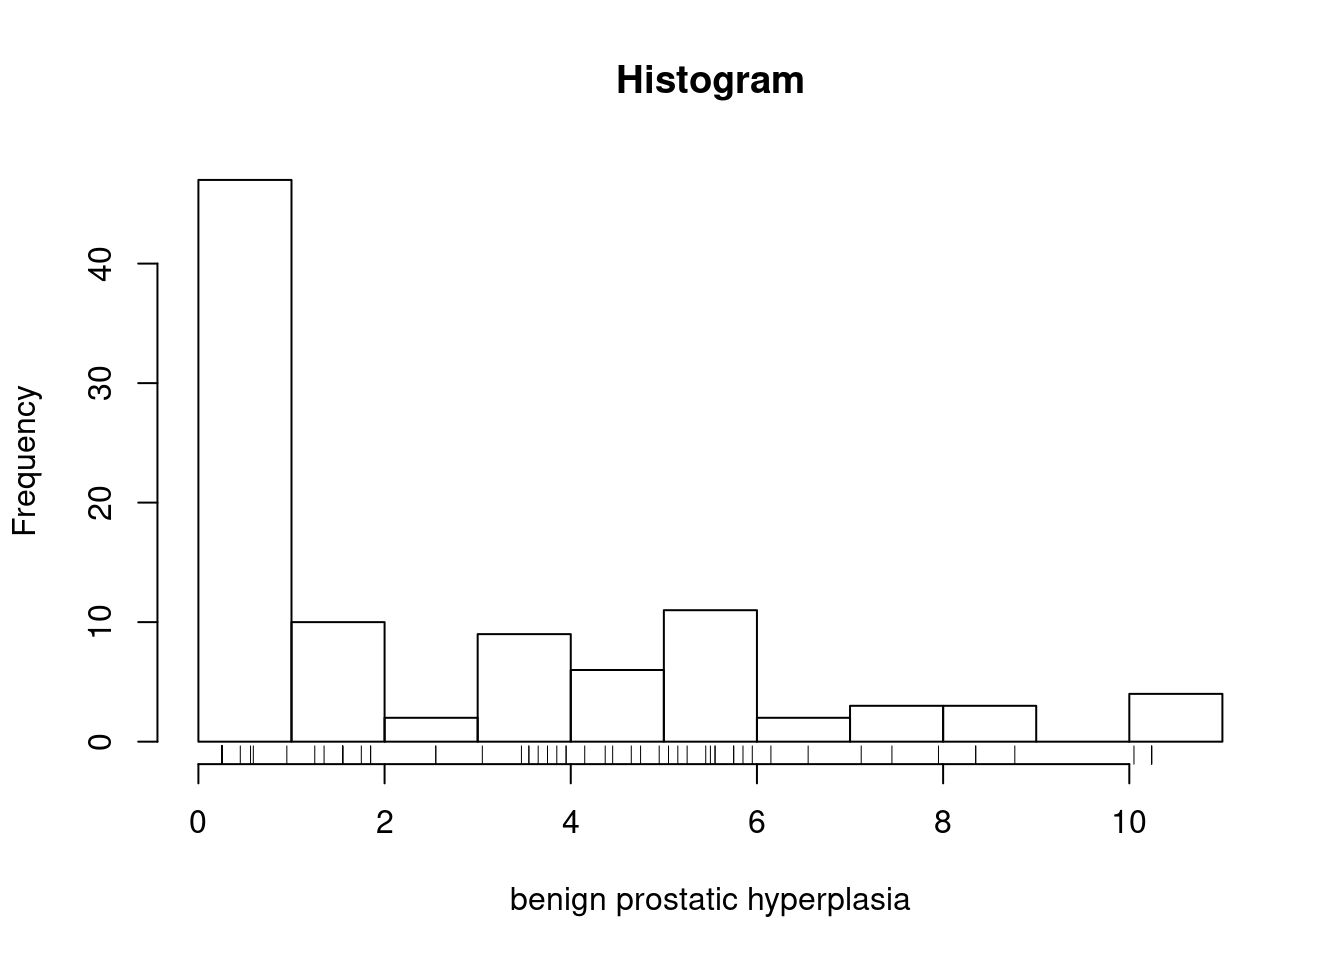
\includegraphics{LinesRModels_files/figure-latex/prostate_question_b2-1.pdf}

\begin{Shaded}
\begin{Highlighting}[]
\CommentTok{#histogram, with lines below where the observations are}
\end{Highlighting}
\end{Shaded}

It seems likely that in order to take a logarithm, zeros were changed to
0.25. As such, we have to be careful with the interpretation of this
coefficient if we include \texttt{bph} in the regression.

\begin{enumerate}
\def\labelenumi{\alph{enumi}.}
\setcounter{enumi}{1}
\tightlist
\item
  Produce a plot of the pair of variables \texttt{lcavol} and
  \texttt{lpsa} on the log and on the original scale. Comment on the
  relationship between \texttt{lcavol} and \texttt{lpsa}.
\end{enumerate}

\begin{Shaded}
\begin{Highlighting}[]
\KeywordTok{par}\NormalTok{(}\DataTypeTok{mfrow =} \KeywordTok{c}\NormalTok{(}\DecValTok{1}\NormalTok{, }\DecValTok{2}\NormalTok{)) }\CommentTok{#graphical parameters: two graphs per window}
\CommentTok{#Function plot is plot(x = , y = ) or plot(y ~ x)}
\CommentTok{#this works for vectors! (error message otherwise)}
\KeywordTok{plot}\NormalTok{(}\KeywordTok{exp}\NormalTok{(lcavol) }\OperatorTok{~}\StringTok{ }\KeywordTok{exp}\NormalTok{(lpsa),}
\DataTypeTok{ylab =} \StringTok{"Cancer volume (milliliters per cc)"}\NormalTok{, }\CommentTok{#y-axis label}
\DataTypeTok{xlab =} \StringTok{"prostate specific antigen (ng/ml)"}\NormalTok{, }\CommentTok{#x-axis label}
\DataTypeTok{main =} \StringTok{"Prostate cancer dataset"}\NormalTok{, }\CommentTok{#title}
\DataTypeTok{bty =} \StringTok{"l"}\NormalTok{, }\DataTypeTok{pch =} \DecValTok{20}\NormalTok{) }\CommentTok{#bty: remove box, only x-y axis}
\CommentTok{#pch: type of plotting symbol (small filled circle)}
\KeywordTok{plot}\NormalTok{(}\DataTypeTok{y =}\NormalTok{ lcavol, }\DataTypeTok{x =}\NormalTok{ lpsa,}
\DataTypeTok{ylab =} \StringTok{"cancer volume (milliliters per cc), log scale"}\NormalTok{,}
\DataTypeTok{xlab =} \StringTok{"prostate specific antigen (ng/ml), log scale"}\NormalTok{, }
\DataTypeTok{main =} \StringTok{"Prostate cancer dataset"}\NormalTok{,}
\DataTypeTok{bty =} \StringTok{"l"}\NormalTok{, }\DataTypeTok{pch =} \DecValTok{20}\NormalTok{)}

\KeywordTok{hist}\NormalTok{(}\KeywordTok{exp}\NormalTok{(lcavol), }\DataTypeTok{xlab =} \StringTok{"cancer volume (milliliters per cc)"}\NormalTok{, }\DataTypeTok{main =} \StringTok{"Histogram"}\NormalTok{)}
\KeywordTok{rug}\NormalTok{(}\KeywordTok{exp}\NormalTok{(lcavol))}
\KeywordTok{hist}\NormalTok{(}\KeywordTok{exp}\NormalTok{(lpsa), }\DataTypeTok{xlab =} \StringTok{"prostate specific antigen (ng/ml)"}\NormalTok{, }\DataTypeTok{main =} \StringTok{"Histogram"}\NormalTok{)}
\KeywordTok{rug}\NormalTok{(}\KeywordTok{exp}\NormalTok{(lpsa))}
\end{Highlighting}
\end{Shaded}

With \texttt{ggplot2}, the same graphs

\begin{Shaded}
\begin{Highlighting}[]
\KeywordTok{library}\NormalTok{(ggplot2)}

\KeywordTok{ggplot}\NormalTok{(}\DataTypeTok{data =}\NormalTok{ prostate, }\KeywordTok{aes}\NormalTok{(}\DataTypeTok{y =}\NormalTok{ lcavol, }\DataTypeTok{x =}\NormalTok{ lpsa)) }\OperatorTok{+}\StringTok{ }
\StringTok{  }\KeywordTok{geom_point}\NormalTok{() }\OperatorTok{+}
\StringTok{  }\KeywordTok{labs}\NormalTok{(}\DataTypeTok{x =} \StringTok{"prostate specific antigen (ng/ml), log scale"}\NormalTok{,}
       \DataTypeTok{y =} \StringTok{"cancer volume (milliliters per cc), log scale"}\NormalTok{,}
       \DataTypeTok{title =} \StringTok{"Prostate cancer dataset"}\NormalTok{)}
\end{Highlighting}
\end{Shaded}

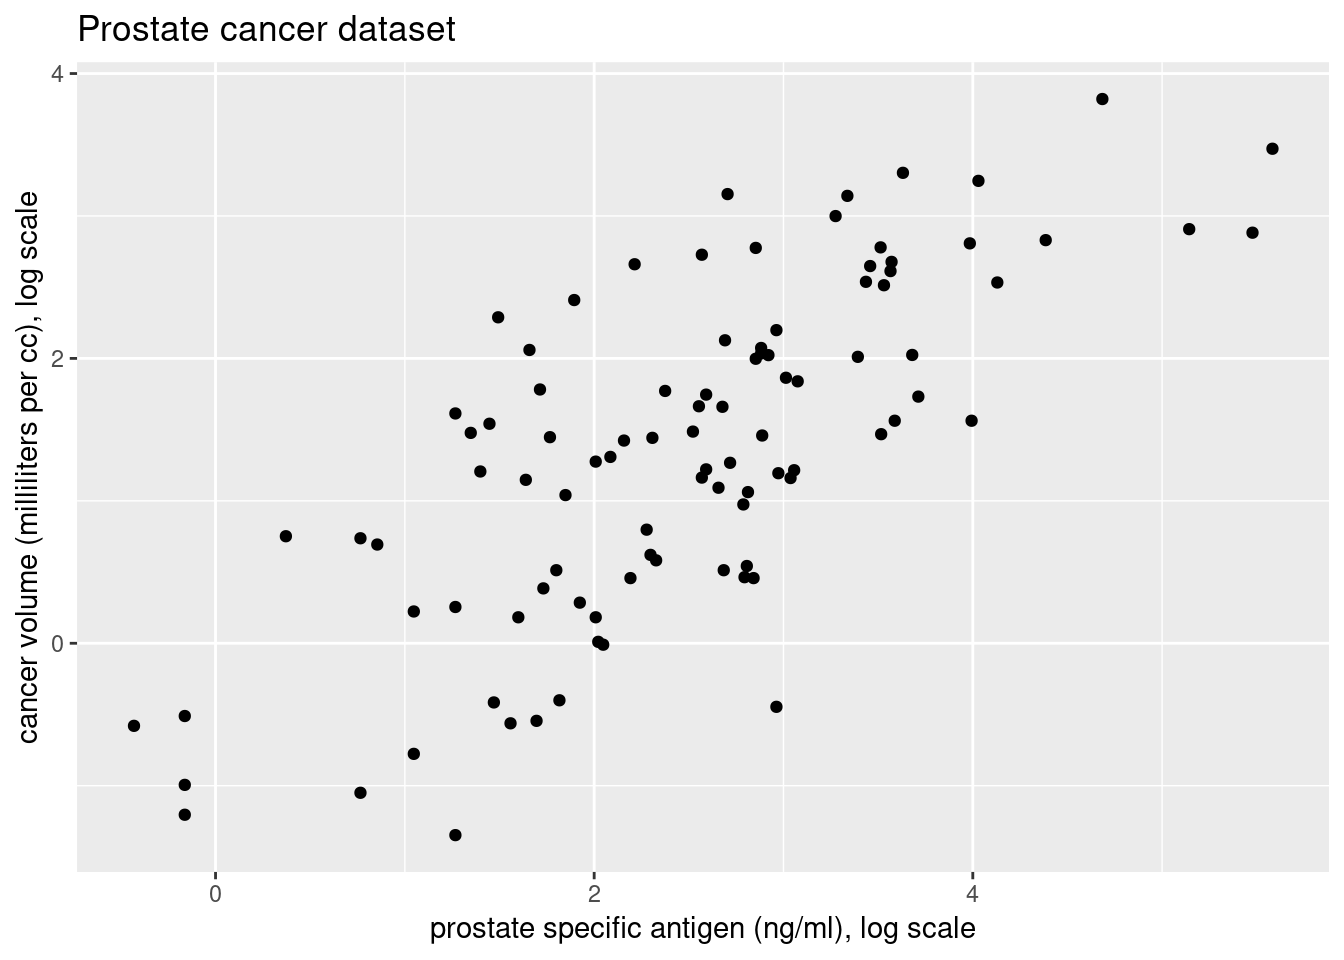
\includegraphics{LinesRModels_files/figure-latex/unnamed-chunk-7-1.pdf}

\begin{Shaded}
\begin{Highlighting}[]
\KeywordTok{ggplot}\NormalTok{(}\DataTypeTok{data =}\NormalTok{ prostate, }\KeywordTok{aes}\NormalTok{(}\DataTypeTok{y =} \KeywordTok{exp}\NormalTok{(lcavol), }\DataTypeTok{x =} \KeywordTok{exp}\NormalTok{(lpsa))) }\OperatorTok{+}\StringTok{ }
\StringTok{  }\KeywordTok{geom_point}\NormalTok{() }\OperatorTok{+}
\StringTok{  }\KeywordTok{labs}\NormalTok{(}\DataTypeTok{x =} \StringTok{"prostate specific antigen (ng/ml)"}\NormalTok{,}
       \DataTypeTok{y =} \StringTok{"cancer volume (milliliters per cc)"}\NormalTok{,}
       \DataTypeTok{title =} \StringTok{"Prostate cancer dataset"}\NormalTok{)}
\end{Highlighting}
\end{Shaded}

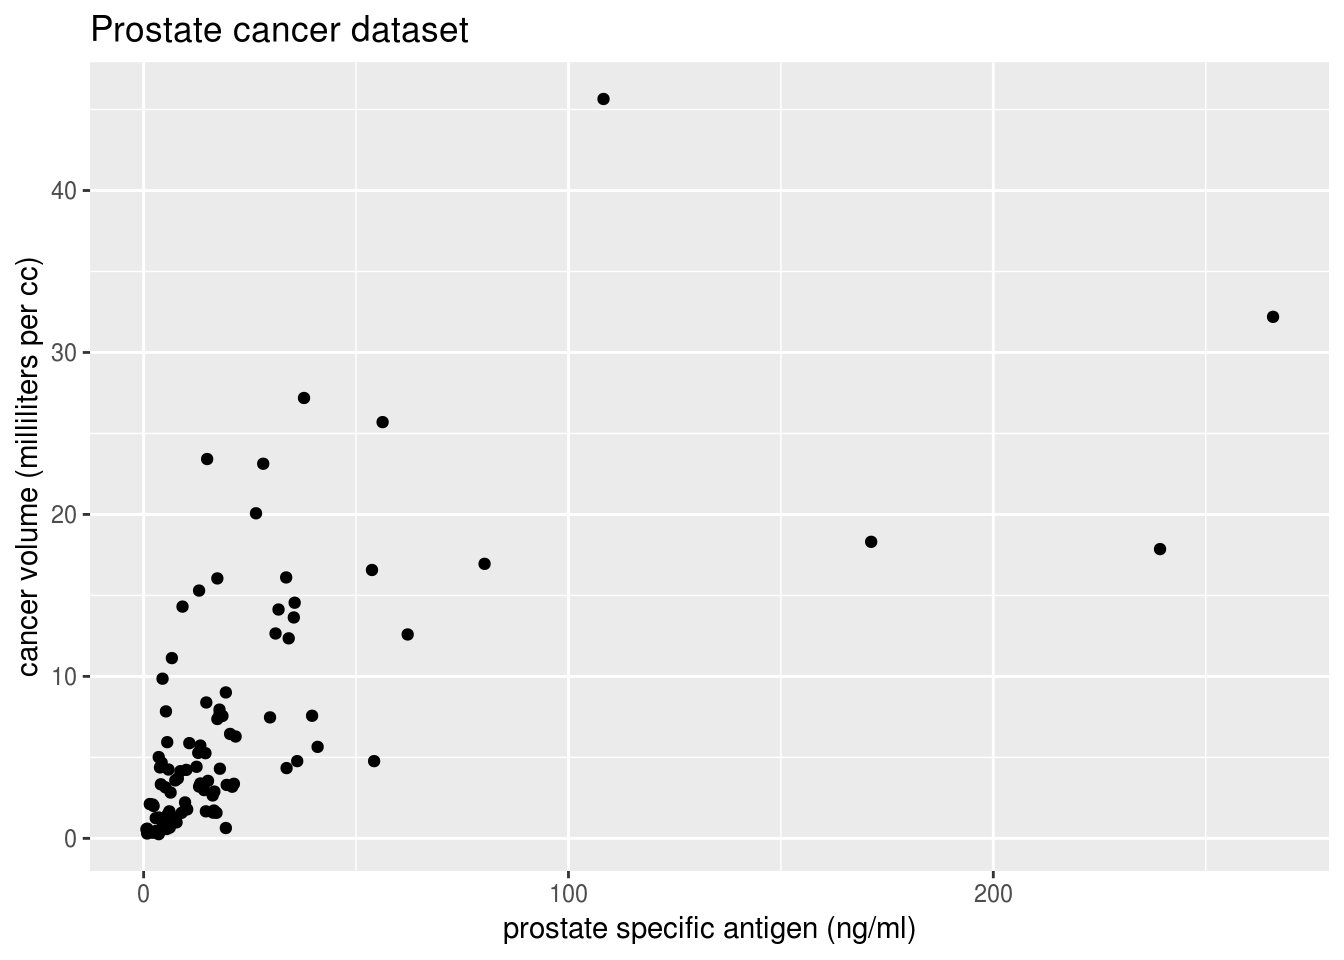
\includegraphics{LinesRModels_files/figure-latex/unnamed-chunk-7-2.pdf}

\begin{Shaded}
\begin{Highlighting}[]
\KeywordTok{ggplot}\NormalTok{(}\DataTypeTok{data =}\NormalTok{ prostate, }\KeywordTok{aes}\NormalTok{(}\DataTypeTok{x =} \KeywordTok{exp}\NormalTok{(lcavol))) }\OperatorTok{+}\StringTok{ }
\StringTok{  }\KeywordTok{geom_histogram}\NormalTok{(}\DataTypeTok{bins =} \DecValTok{30}\NormalTok{) }\OperatorTok{+}\StringTok{ }\KeywordTok{geom_rug}\NormalTok{() }\OperatorTok{+}\StringTok{ }
\StringTok{  }\KeywordTok{labs}\NormalTok{(}\DataTypeTok{x =} \StringTok{"cancer volume (milliliters per cc)"}\NormalTok{,}
       \DataTypeTok{title =} \StringTok{"Histogram"}\NormalTok{)}
\end{Highlighting}
\end{Shaded}

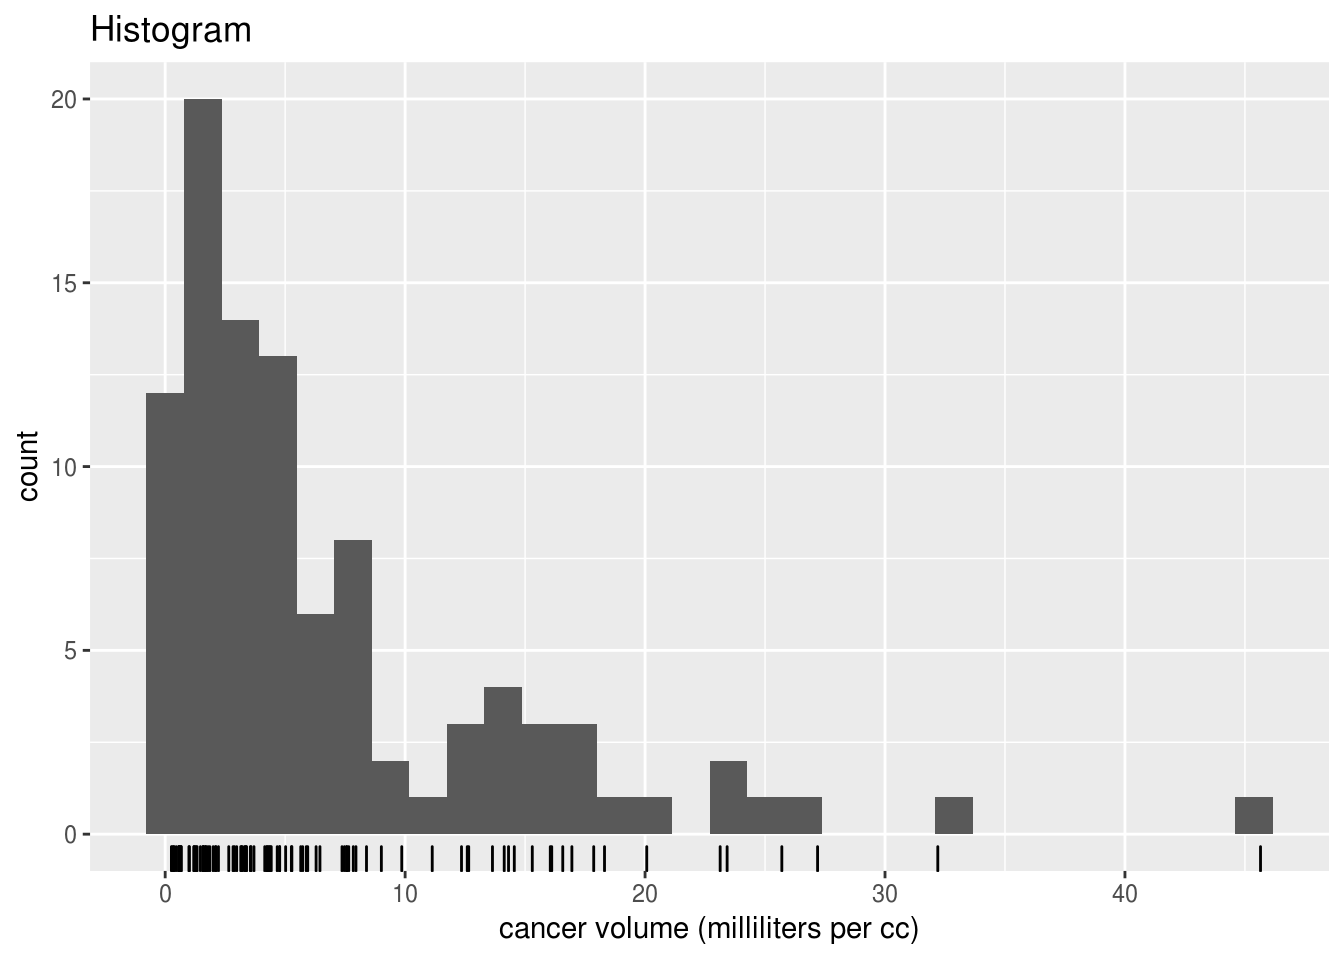
\includegraphics{LinesRModels_files/figure-latex/unnamed-chunk-7-3.pdf}

We can see that both variables are positive and positively skewed, so a
log transform may lead to a more linear relationship, as indicated by
the pairs plot. A multiplicative model on the original scale is thus
reasonable.

\begin{enumerate}
\def\labelenumi{\alph{enumi}.}
\setcounter{enumi}{3}
\tightlist
\item
  Fit a linear model using the log cancer volume as response variable,
  including a constant and the log prostate specific antigen as
  covariates. Obtain numerically the OLS estimates
  \(\hat{\boldsymbol{\beta}}\) of the parameters, the fitted values
  \(\hat{\boldsymbol{y}}\) and the residuals \(\boldsymbol{e}\) using
  the formulae given in class.
\end{enumerate}

\begin{Shaded}
\begin{Highlighting}[]
\NormalTok{fit <-}\StringTok{ }\KeywordTok{lm}\NormalTok{(lcavol }\OperatorTok{~}\StringTok{ }\NormalTok{lpsa, }\DataTypeTok{data =}\NormalTok{ prostate)}
\KeywordTok{summary}\NormalTok{(fit)}
\end{Highlighting}
\end{Shaded}

\begin{verbatim}
## 
## Call:
## lm(formula = lcavol ~ lpsa, data = prostate)
## 
## Residuals:
##      Min       1Q   Median       3Q      Max 
## -2.15949 -0.59384  0.05034  0.50826  1.67751 
## 
## Coefficients:
##             Estimate Std. Error t value Pr(>|t|)    
## (Intercept) -0.50858    0.19419  -2.619   0.0103 *  
## lpsa         0.74992    0.07109  10.548   <2e-16 ***
## ---
## Signif. codes:  0 '***' 0.001 '**' 0.01 '*' 0.05 '.' 0.1 ' ' 1
## 
## Residual standard error: 0.8041 on 95 degrees of freedom
## Multiple R-squared:  0.5394, Adjusted R-squared:  0.5346 
## F-statistic: 111.3 on 1 and 95 DF,  p-value: < 2.2e-16
\end{verbatim}

\begin{Shaded}
\begin{Highlighting}[]
\CommentTok{#Create response vector and design matrix}
\NormalTok{y <-}\StringTok{ }\NormalTok{lcavol}
\NormalTok{X <-}\StringTok{ }\KeywordTok{cbind}\NormalTok{(}\DecValTok{1}\NormalTok{, lpsa)}
\CommentTok{#Create function to compute coefs "by hand"}
\NormalTok{coefs_vals <-}\StringTok{ }\ControlFlowTok{function}\NormalTok{(x, y)\{}
  \KeywordTok{c}\NormalTok{(}\KeywordTok{solve}\NormalTok{(}\KeywordTok{crossprod}\NormalTok{(x), }\KeywordTok{crossprod}\NormalTok{(x, y)))}
\NormalTok{\}}
\CommentTok{# Compute coefficients, fitted values and residuals}
\NormalTok{beta_hat <-}\StringTok{ }\KeywordTok{coefs_vals}\NormalTok{(}\DataTypeTok{x =}\NormalTok{ X, }\DataTypeTok{y =}\NormalTok{ lcavol)}
\NormalTok{yhat <-}\StringTok{ }\KeywordTok{c}\NormalTok{(X }\OperatorTok\StringTok{ }\NormalTok{beta_hat)}
\NormalTok{e <-}\StringTok{ }\NormalTok{y }\OperatorTok{-}\StringTok{ }\NormalTok{yhat}
\end{Highlighting}
\end{Shaded}

The function \texttt{lm} fits a linear model by least squares to a
dataset. The function \texttt{summary} will return coefficient
estimates, standard errors and various other statistics formatted in a
way so that they can be printed to the console.

The formula for \texttt{lm} must be of the form
\texttt{y\ \textasciitilde{}}, and any combination of the variables
appearing on the right hand side of the \texttt{\textasciitilde{}} will
be added as new columns of the design matrix. By default, the latter
includes a column of ones. To remove it, use \texttt{+0} or \texttt{-1}.
If you have two covariates \texttt{x1} and \texttt{x2}, the model
\texttt{x1+x2} will have for \(i\)th row \((1, x_{i1}, x_{i2})\), while
the model \texttt{x1+x2+x1:x2}\(\equiv\)\texttt{x1*x2} will include an
\emph{interaction} term \texttt{x1:x2}. The latter just means product,
so the \(i\)th row of the design matrix would be
\((1, x_{i1}, x_{i2}, x_{i1}x_{i2})\). \textbf{R} will drop any
collinear vectors, warn you and report \texttt{NA} in the summary
output.

\begin{enumerate}
\def\labelenumi{\alph{enumi}.}
\setcounter{enumi}{4}
\tightlist
\item
  Compare the quantities you obtained in the last question with the
  output of the function \texttt{lm}.
\end{enumerate}

\begin{Shaded}
\begin{Highlighting}[]
\NormalTok{beta_hat }\CommentTok{# equivalent to print(beta_hat)}
\end{Highlighting}
\end{Shaded}

\begin{verbatim}
## [1] -0.5085796  0.7499189
\end{verbatim}

\begin{Shaded}
\begin{Highlighting}[]
\KeywordTok{coef}\NormalTok{(fit) }\CommentTok{# coefficients from object of class `lm`}
\end{Highlighting}
\end{Shaded}

\begin{verbatim}
## (Intercept)        lpsa 
##  -0.5085796   0.7499189
\end{verbatim}

\begin{Shaded}
\begin{Highlighting}[]
\KeywordTok{isTRUE}\NormalTok{(}\KeywordTok{all.equal}\NormalTok{(beta_hat, }\KeywordTok{coef}\NormalTok{(fit), }\DataTypeTok{check.attributes =} \OtherTok{FALSE}\NormalTok{))}
\end{Highlighting}
\end{Shaded}

\begin{verbatim}
## [1] TRUE
\end{verbatim}

\begin{Shaded}
\begin{Highlighting}[]
\KeywordTok{isTRUE}\NormalTok{(}\KeywordTok{all.equal}\NormalTok{(}\KeywordTok{c}\NormalTok{(yhat), }\KeywordTok{fitted}\NormalTok{(fit), }\DataTypeTok{check.attributes =} \OtherTok{FALSE}\NormalTok{))}
\end{Highlighting}
\end{Shaded}

\begin{verbatim}
## [1] TRUE
\end{verbatim}

\begin{Shaded}
\begin{Highlighting}[]
\KeywordTok{isTRUE}\NormalTok{(}\KeywordTok{all.equal}\NormalTok{(e, }\KeywordTok{resid}\NormalTok{(fit), }\DataTypeTok{check.attributes =} \OtherTok{FALSE}\NormalTok{))}
\end{Highlighting}
\end{Shaded}

\begin{verbatim}
## [1] TRUE
\end{verbatim}

\begin{enumerate}
\def\labelenumi{\alph{enumi}.}
\setcounter{enumi}{5}
\tightlist
\item
  Add the fitted regression line to the scatterplot of lcavol against
  lpsa .
\end{enumerate}

\begin{Shaded}
\begin{Highlighting}[]
\KeywordTok{par}\NormalTok{(}\DataTypeTok{mfrow =} \KeywordTok{c}\NormalTok{(}\DecValTok{1}\NormalTok{, }\DecValTok{1}\NormalTok{))}
\KeywordTok{plot}\NormalTok{(lcavol }\OperatorTok{~}\StringTok{ }\NormalTok{lpsa, }\DataTypeTok{data =}\NormalTok{ prostate,}
  \DataTypeTok{ylab =} \StringTok{"Cancer volume (milliliters per cc), log scale"}\NormalTok{,}
  \DataTypeTok{xlab =} \StringTok{"prostate specific antigen (ng/ml), log scale"}\NormalTok{, }
  \DataTypeTok{main =} \StringTok{"Prostate cancer dataset"}\NormalTok{,}
  \DataTypeTok{bty =} \StringTok{"l"}\NormalTok{, }\DataTypeTok{pch =} \DecValTok{20}\NormalTok{)}
\KeywordTok{abline}\NormalTok{(fit, }\DataTypeTok{lwd =} \DecValTok{2}\NormalTok{) }\CommentTok{#simply add regression line, lwd is line width}
\end{Highlighting}
\end{Shaded}

\begin{Shaded}
\begin{Highlighting}[]
\KeywordTok{ggplot}\NormalTok{(}\DataTypeTok{data =}\NormalTok{ prostate, }\KeywordTok{aes}\NormalTok{(}\DataTypeTok{y =}\NormalTok{ lcavol, }\DataTypeTok{x =}\NormalTok{ lpsa)) }\OperatorTok{+}\StringTok{ }
\StringTok{  }\KeywordTok{geom_point}\NormalTok{() }\OperatorTok{+}
\StringTok{  }\KeywordTok{labs}\NormalTok{(}\DataTypeTok{x =} \StringTok{"prostate specific antigen (ng/ml), log scale"}\NormalTok{,}
       \DataTypeTok{y =} \StringTok{"cancer volume (milliliters per cc), log scale"}\NormalTok{,}
       \DataTypeTok{title =} \StringTok{"Prostate cancer dataset"}\NormalTok{) }\OperatorTok{+}\StringTok{ }
\StringTok{  }\KeywordTok{geom_smooth}\NormalTok{(}\DataTypeTok{method =} \StringTok{"lm"}\NormalTok{, }\DataTypeTok{se =} \OtherTok{FALSE}\NormalTok{)}
\end{Highlighting}
\end{Shaded}

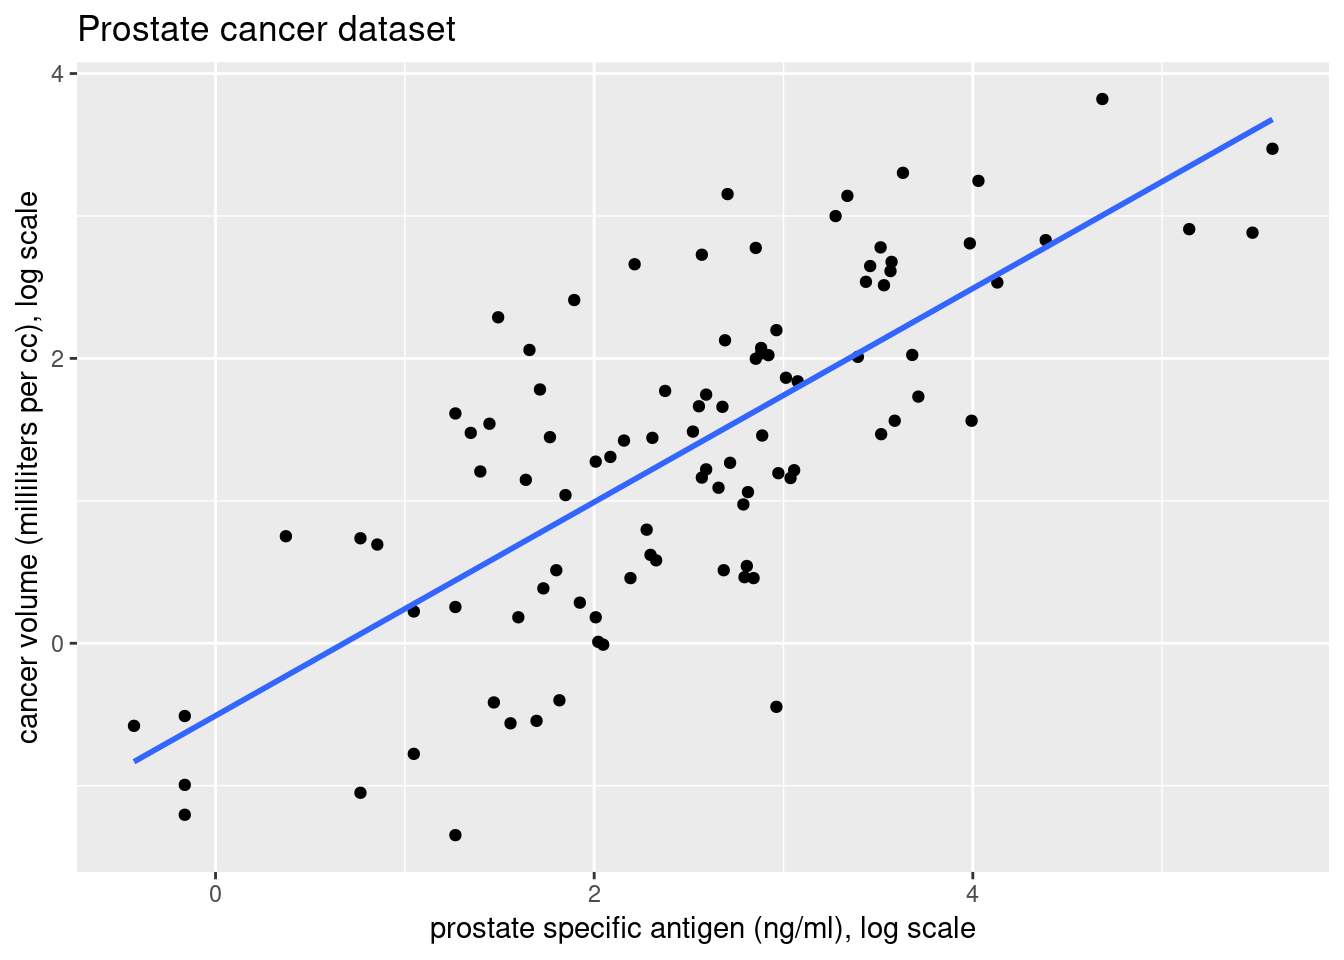
\includegraphics{LinesRModels_files/figure-latex/question_eggplot2-1.pdf}

\begin{enumerate}
\def\labelenumi{\alph{enumi}.}
\setcounter{enumi}{6}
\tightlist
\item
  Interpret the changes in cancer volume (not the log cancer volume),
  including any units in your interpretations.
\end{enumerate}

The interpretation is as follows. We fit
\[\log(\texttt{cavol}_i) = \beta_0 + \beta_1 \log(\texttt{psa}_i) + \varepsilon_i.\]

On the original scale, this translates into the multiplicative model
\(\texttt{cavol}_i= \exp^{\beta_0}\texttt{psa}_i^{\beta_1}\exp(\varepsilon_i)\).
The effect of an increase of one ng/mll of prostate specific antigen
depends on the specific level of \(\texttt{psa}\),
\((\texttt{psa}_1/\texttt{psa}_2)^{\beta_1}\) for levels
\(\texttt{psa}_1\) and \(\texttt{psa}_2\). For example, an increase of
the PSA level from 5.25 ng/mll to 6.15 ng/mll leads an increase of the
volume of cancer of prostate cancer of 1.13 milliliters per cubic
centimeter.

\begin{enumerate}
\def\labelenumi{\alph{enumi}.}
\setcounter{enumi}{7}
\tightlist
\item
  Using the results of Exercise 4.2, obtain the orthogonal projection
  matrix \(\mathbf{H}_{\mathbf{X}}\) and \(\hat{\boldsymbol{\beta}}\)
  using a SVD decomposition (\texttt{svd}). Check your output.
\end{enumerate}

\begin{Shaded}
\begin{Highlighting}[]
\CommentTok{#Hat matrix}
\NormalTok{Hmat <-}\StringTok{ }\NormalTok{X }\OperatorTok\StringTok{ }\KeywordTok{solve}\NormalTok{(}\KeywordTok{crossprod}\NormalTok{(X)) }\OperatorTok\StringTok{ }\KeywordTok{t}\NormalTok{(X)}
\CommentTok{#SVD decomposition of X}
\NormalTok{svdX <-}\StringTok{ }\KeywordTok{svd}\NormalTok{(X)}
\CommentTok{#OLS coefficients}
\NormalTok{beta_hat_svd <-}\StringTok{ }\NormalTok{svdX}\OperatorTok{$}\NormalTok{v }\OperatorTok\StringTok{ }\NormalTok{(}\KeywordTok{t}\NormalTok{(svdX}\OperatorTok{$}\NormalTok{u) }\OperatorTok\StringTok{ }\NormalTok{lcavol }\OperatorTok{/}\StringTok{ }\NormalTok{svdX}\OperatorTok{$}\NormalTok{d)}
\NormalTok{Hmat_svd <-}\StringTok{ }\KeywordTok{tcrossprod}\NormalTok{(svdX}\OperatorTok{$}\NormalTok{u)}
\CommentTok{#Check that both quantities are equal}
\KeywordTok{all.equal}\NormalTok{(Hmat, Hmat_svd, }\DataTypeTok{check.attributes =} \OtherTok{FALSE}\NormalTok{) }
\end{Highlighting}
\end{Shaded}

\begin{verbatim}
## [1] TRUE
\end{verbatim}

\begin{Shaded}
\begin{Highlighting}[]
\CommentTok{#use check.attributes = FALSE }
\CommentTok{#if you want to compare only the values}
\CommentTok{#and not e.g. the column names}
\KeywordTok{all.equal}\NormalTok{(}\KeywordTok{c}\NormalTok{(beta_hat_svd), beta_hat)}
\end{Highlighting}
\end{Shaded}

\begin{verbatim}
## [1] TRUE
\end{verbatim}

\begin{enumerate}
\def\labelenumi{\roman{enumi}.}
\tightlist
\item
  Compute the \(R^2_c\) coefficient and compare with the one in summary
  output of the \texttt{lm} function. What can you say about the
  explanatory power of the covariate \texttt{lpsa} ?
\end{enumerate}

\begin{Shaded}
\begin{Highlighting}[]
\NormalTok{R2c <-}\StringTok{ }\KeywordTok{sum}\NormalTok{((yhat}\OperatorTok{-}\KeywordTok{mean}\NormalTok{(y))}\OperatorTok{^}\DecValTok{2}\NormalTok{)}\OperatorTok{/}\KeywordTok{sum}\NormalTok{((y}\OperatorTok{-}\KeywordTok{mean}\NormalTok{(y))}\OperatorTok{^}\DecValTok{2}\NormalTok{)}
\NormalTok{R2c_lm <-}\StringTok{ }\KeywordTok{summary}\NormalTok{(fit)}\OperatorTok{$}\NormalTok{r.squared }\CommentTok{#this is centered version}
\KeywordTok{all.equal}\NormalTok{(R2c, R2c_lm)}
\end{Highlighting}
\end{Shaded}

\begin{verbatim}
## [1] TRUE
\end{verbatim}

\begin{Shaded}
\begin{Highlighting}[]
\CommentTok{#Detach prostate from environment}
\KeywordTok{detach}\NormalTok{(prostate)}
\end{Highlighting}
\end{Shaded}

The value of \(R^2_c\) is about 0.54, so about half the variability can
be explained by the model. There is reasonable explanatory power. Note
that presence of cancer causes the prostate specific antigens to
increase (not the other way around!) so be careful in your
interpretation. A linear model could nevertheless be sensible here if we
wished to obtain a non-invasive detector for predicting presence/absence
of cancer, assuming the antigen is present in blood samples, but that
detection of cancer would require otherwise a biopsy.

\hypertarget{frischwaughlovell-theorem}{%
\chapter{Frisch--Waugh--Lovell
theorem}\label{frischwaughlovell-theorem}}

This result dates back to the work of
\href{https://www.jstor.org/stable/1907330}{Frisch, R. and F. Waugh
(1933)} and of \href{https://doi.org/10.1080/01621459.1963.10480682}{M.
Lovell (1963)}. The FWL theorem has two components: it gives a formula
for partitioned OLS estimates and shows that residuals from sequential
regressions are identical.

Consider the following linear regression \[
 {\boldsymbol{y}}= {\mathbf{X}}_1\boldsymbol{\beta}_1+{\mathbf{X}}_2\boldsymbol{\beta}_2+ \boldsymbol{u}, \label{eq1}
\] where the response vector \({\boldsymbol{y}}\) is \(n \times 1\), the
vector of errors \(\boldsymbol{u}\) is a realization from a mean zero
random variable. The \(n \times p\) full-rank design matrix
\({\mathbf{X}}\) can be written as the partitioned matrix
\(({\mathbf{X}}_1^\top, {\mathbf{X}}_2^\top)^\top\) with blocks
\({\mathbf{X}}_1\), an \(n \times p_1\) matrix, and \({\mathbf{X}}_2\),
an \(n \times p_2\) matrix. Let \(\hat{\boldsymbol{\beta}}_1\) and
\(\hat{\boldsymbol{\beta}}_2\) be the ordinary least square (OLS)
parameter estimates from running this regression. Define the orthogonal
projection matrix \(\mathbf{H}_{\mathbf{X}}\) as usual and
\(\mathbf{H}_{{\mathbf{X}}_i} = {\mathbf{X}}_i^{\vphantom{\top}}({\mathbf{X}}_i^\top{\mathbf{X}}_i^{\vphantom{\top}})^{-1}{\mathbf{X}}_i^\top\)
for \(i=1, 2\). Similarly, define the complementary projection matrices
\(\mathbf{M}_{{\mathbf{X}}_1}=\mathbf{I}_n-\mathbf{H}_{{\mathbf{X}}_1}\)
and
\(\mathbf{M}_{{\mathbf{X}}_2}=\mathbf{I}_n-\mathbf{H}_{{\mathbf{X}}_2}\).

\BeginKnitrBlock{theorem}
\protect\hypertarget{thm:unnamed-chunk-9}{}{\label{thm:unnamed-chunk-9} }The
ordinary least square estimates of \(\boldsymbol{\beta}_2\) and the
residuals from \eqref{eq1} are identical to those obtained by running
the regression \[
 \mathbf{M}_{{\mathbf{X}}_1}{\boldsymbol{y}}= \mathbf{M}_{{\mathbf{X}}_1}{\mathbf{X}}_2\boldsymbol{\beta}_2 + \text{residuals}. \label{eq2} \
\]
\EndKnitrBlock{theorem}

\BeginKnitrBlock{proof}
\iffalse{} {Proof. } \fi{}The easiest proof uses projection matrices,
but we demonstrate the result for OLS coefficients directly. Consider an
invertible \(d \times d\) matrix \(\mathbf{C}\) and denote its inverse
by \(\mathbf{D}\); then \[
\begin{pmatrix} \mathbf{C}_{11} & \mathbf{C}_{12} \\ \mathbf{C}_{21} &\mathbf{C}_{22}
\end{pmatrix}\begin{pmatrix} \mathbf{D}_{11} & \mathbf{D}_{12} \\ \mathbf{D}_{21} &\mathbf{D}_{22}
\end{pmatrix}
=\mathbf{I}_p
\] gives the relationships \begin{align*}
\mathbf{C}_{11}\mathbf{D}_{11}+\mathbf{C}_{12}\mathbf{D}_{21} &= \mathbf{I}_{p_1}\\
\mathbf{C}_{11}\mathbf{D}_{12}+\mathbf{C}_{12}\mathbf{D}_{22} &= \mathbf{O}_{p_1, p_2}\\
\mathbf{C}_{22}\mathbf{D}_{21}+\mathbf{C}_{21}\mathbf{D}_{11} &= \mathbf{O}_{p_2, p_1}\\
\mathbf{C}_{22}\mathbf{D}_{22}+\mathbf{C}_{21}\mathbf{D}_{12} &= \mathbf{I}_{p_2}\\
\end{align*} from which we deduce that the so-called Schur complement of
\(\mathbf{C}_{22}\) is
\[\mathbf{C}_{11}+\mathbf{C}_{12}\mathbf{C}^{-1}_{22}\mathbf{C}_{21} = \mathbf{D}_{11}^{-1}\]
and \[
-\mathbf{C}_{22}\mathbf{C}_{21}(\mathbf{C}_{11}+\mathbf{C}_{12}\mathbf{C}^{-1}_{22}\mathbf{C}_{21})^{-1} = \mathbf{D}_{21}.
\] Substituting \[
\begin{pmatrix} \mathbf{C}_{11} & \mathbf{C}_{12} \\ \mathbf{C}_{21} &\mathbf{C}_{22}
\end{pmatrix} \equiv \begin{pmatrix} \mathbf{X}_1^\top\mathbf{X}_1 & \mathbf{X}_1^\top\mathbf{X}_2\\\mathbf{X}_2^\top\mathbf{X}_1  &\mathbf{X}_2^\top\mathbf{X}_2 
\end{pmatrix}
\] and plug-in this result back in the equation for the least squares
yields \begin{align*}
\hat{\boldsymbol{\beta}}_1 &= (\mathbf{D}_{11}\mathbf{X}_1^\top + \mathbf{D}_{12}\mathbf{X}_2^\top)\boldsymbol{y} 
\\&= \mathbf{D}_{11}( \mathbf{X}_1^\top - \mathbf{C}_{12}\mathbf{C}_{22}^{-1}\mathbf{X}_2)\boldsymbol{y}
\\&= \left(\mathbf{C}_{11}+\mathbf{C}_{12}\mathbf{C}^{-1}_{22}\mathbf{C}_{21}\right)^{-1} \mathbf{X}_1^\top\mathbf{M}_{\mathbf{X}_2}\boldsymbol{y} 
\\&= (\mathbf{X}_1^\top\mathbf{M}_{\mathbf{X}_2}\mathbf{X}_1)^{-1}\mathbf{X}_1^\top\mathbf{M}_{\mathbf{X}_2}\boldsymbol{y}.
\end{align*}

The proof that the residuals are the same is left as an exercise.
\EndKnitrBlock{proof}

\hypertarget{examples}{%
\section{Examples}\label{examples}}

We have seen last week the centered \(R^2_c\); the latter is equivalent
to the coefficient of determination from the FWL regression
\[ \mathbf{M}_{\mathbf{1}_n}\boldsymbol{y} = \mathbf{M}_{\mathbf{1}_n}\mathbf{X}\boldsymbol{\beta} + \boldsymbol{\varepsilon},\]
that is, after centering regressand and regressors. Note that this
regression will have no intercept, because this coefficient would be
exactly zero.

To be continued.

\bibliography{book.bib,packages.bib}


\end{document}
